%!TEX root = ../xesphVI.tex
\chapter{光波与光线}

\section{界面上的反射与折射}

\subsection{光波与光线}

众所周知,\,光是电磁频谱的一段.\,我们所说的光一般是指\emph{可见光}(visible light),\,学术上代表波长为$400-700{\rm nm}$的电磁辐射.\,它大致代表了人对光的色视觉的界限.\,而一般的光学研究还包括了波长长至$1{\rm mm}$左右的\emph{红外光}(infrared light,\,IR)与短至$10{\rm nm}$的\emph{紫外光}(ultraviolet light,\,UV).
\begin{figure}[H]
\centering
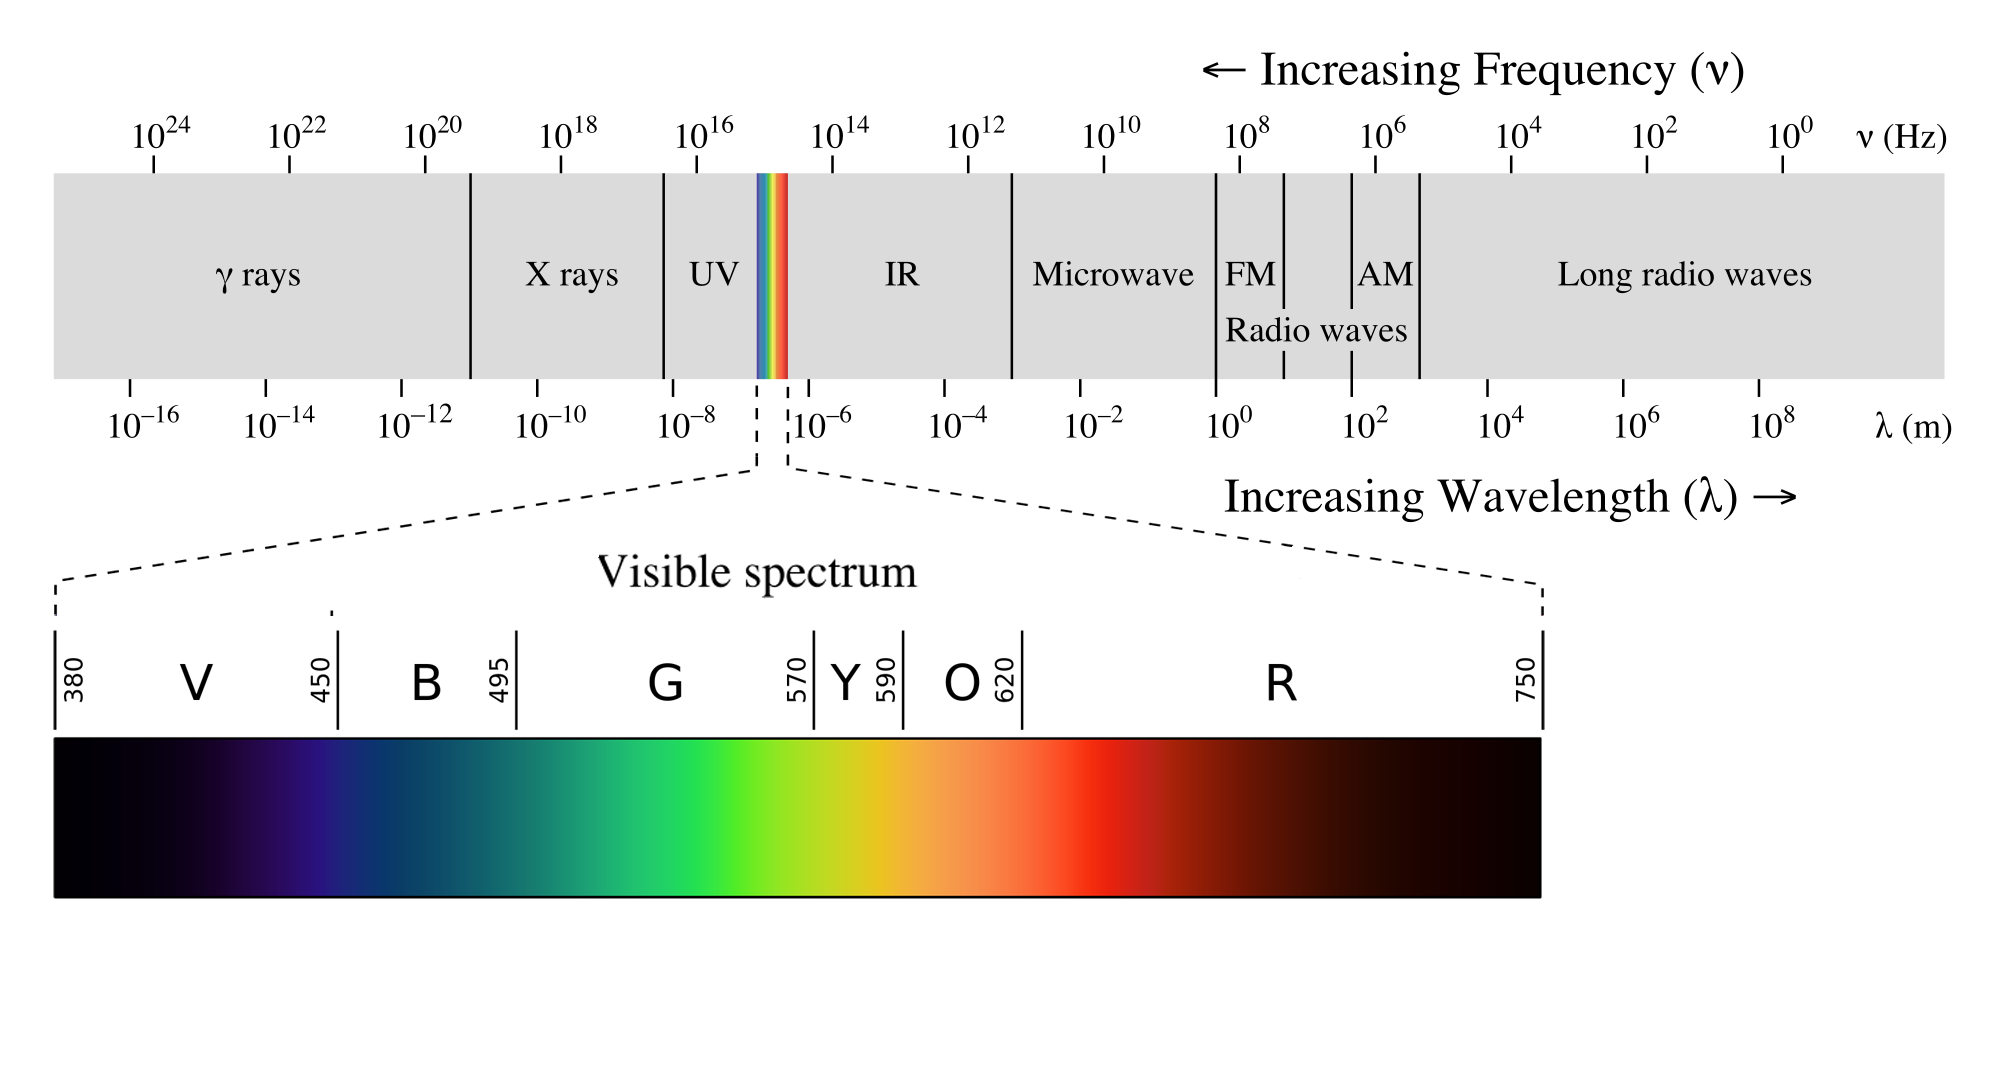
\includegraphics[width=0.8\textwidth]{image/5-6-1.png}
\caption{光学研究范围}
\end{figure}

\begin{wrapfigure}[14]{o}[-10pt]{7cm}
\centering
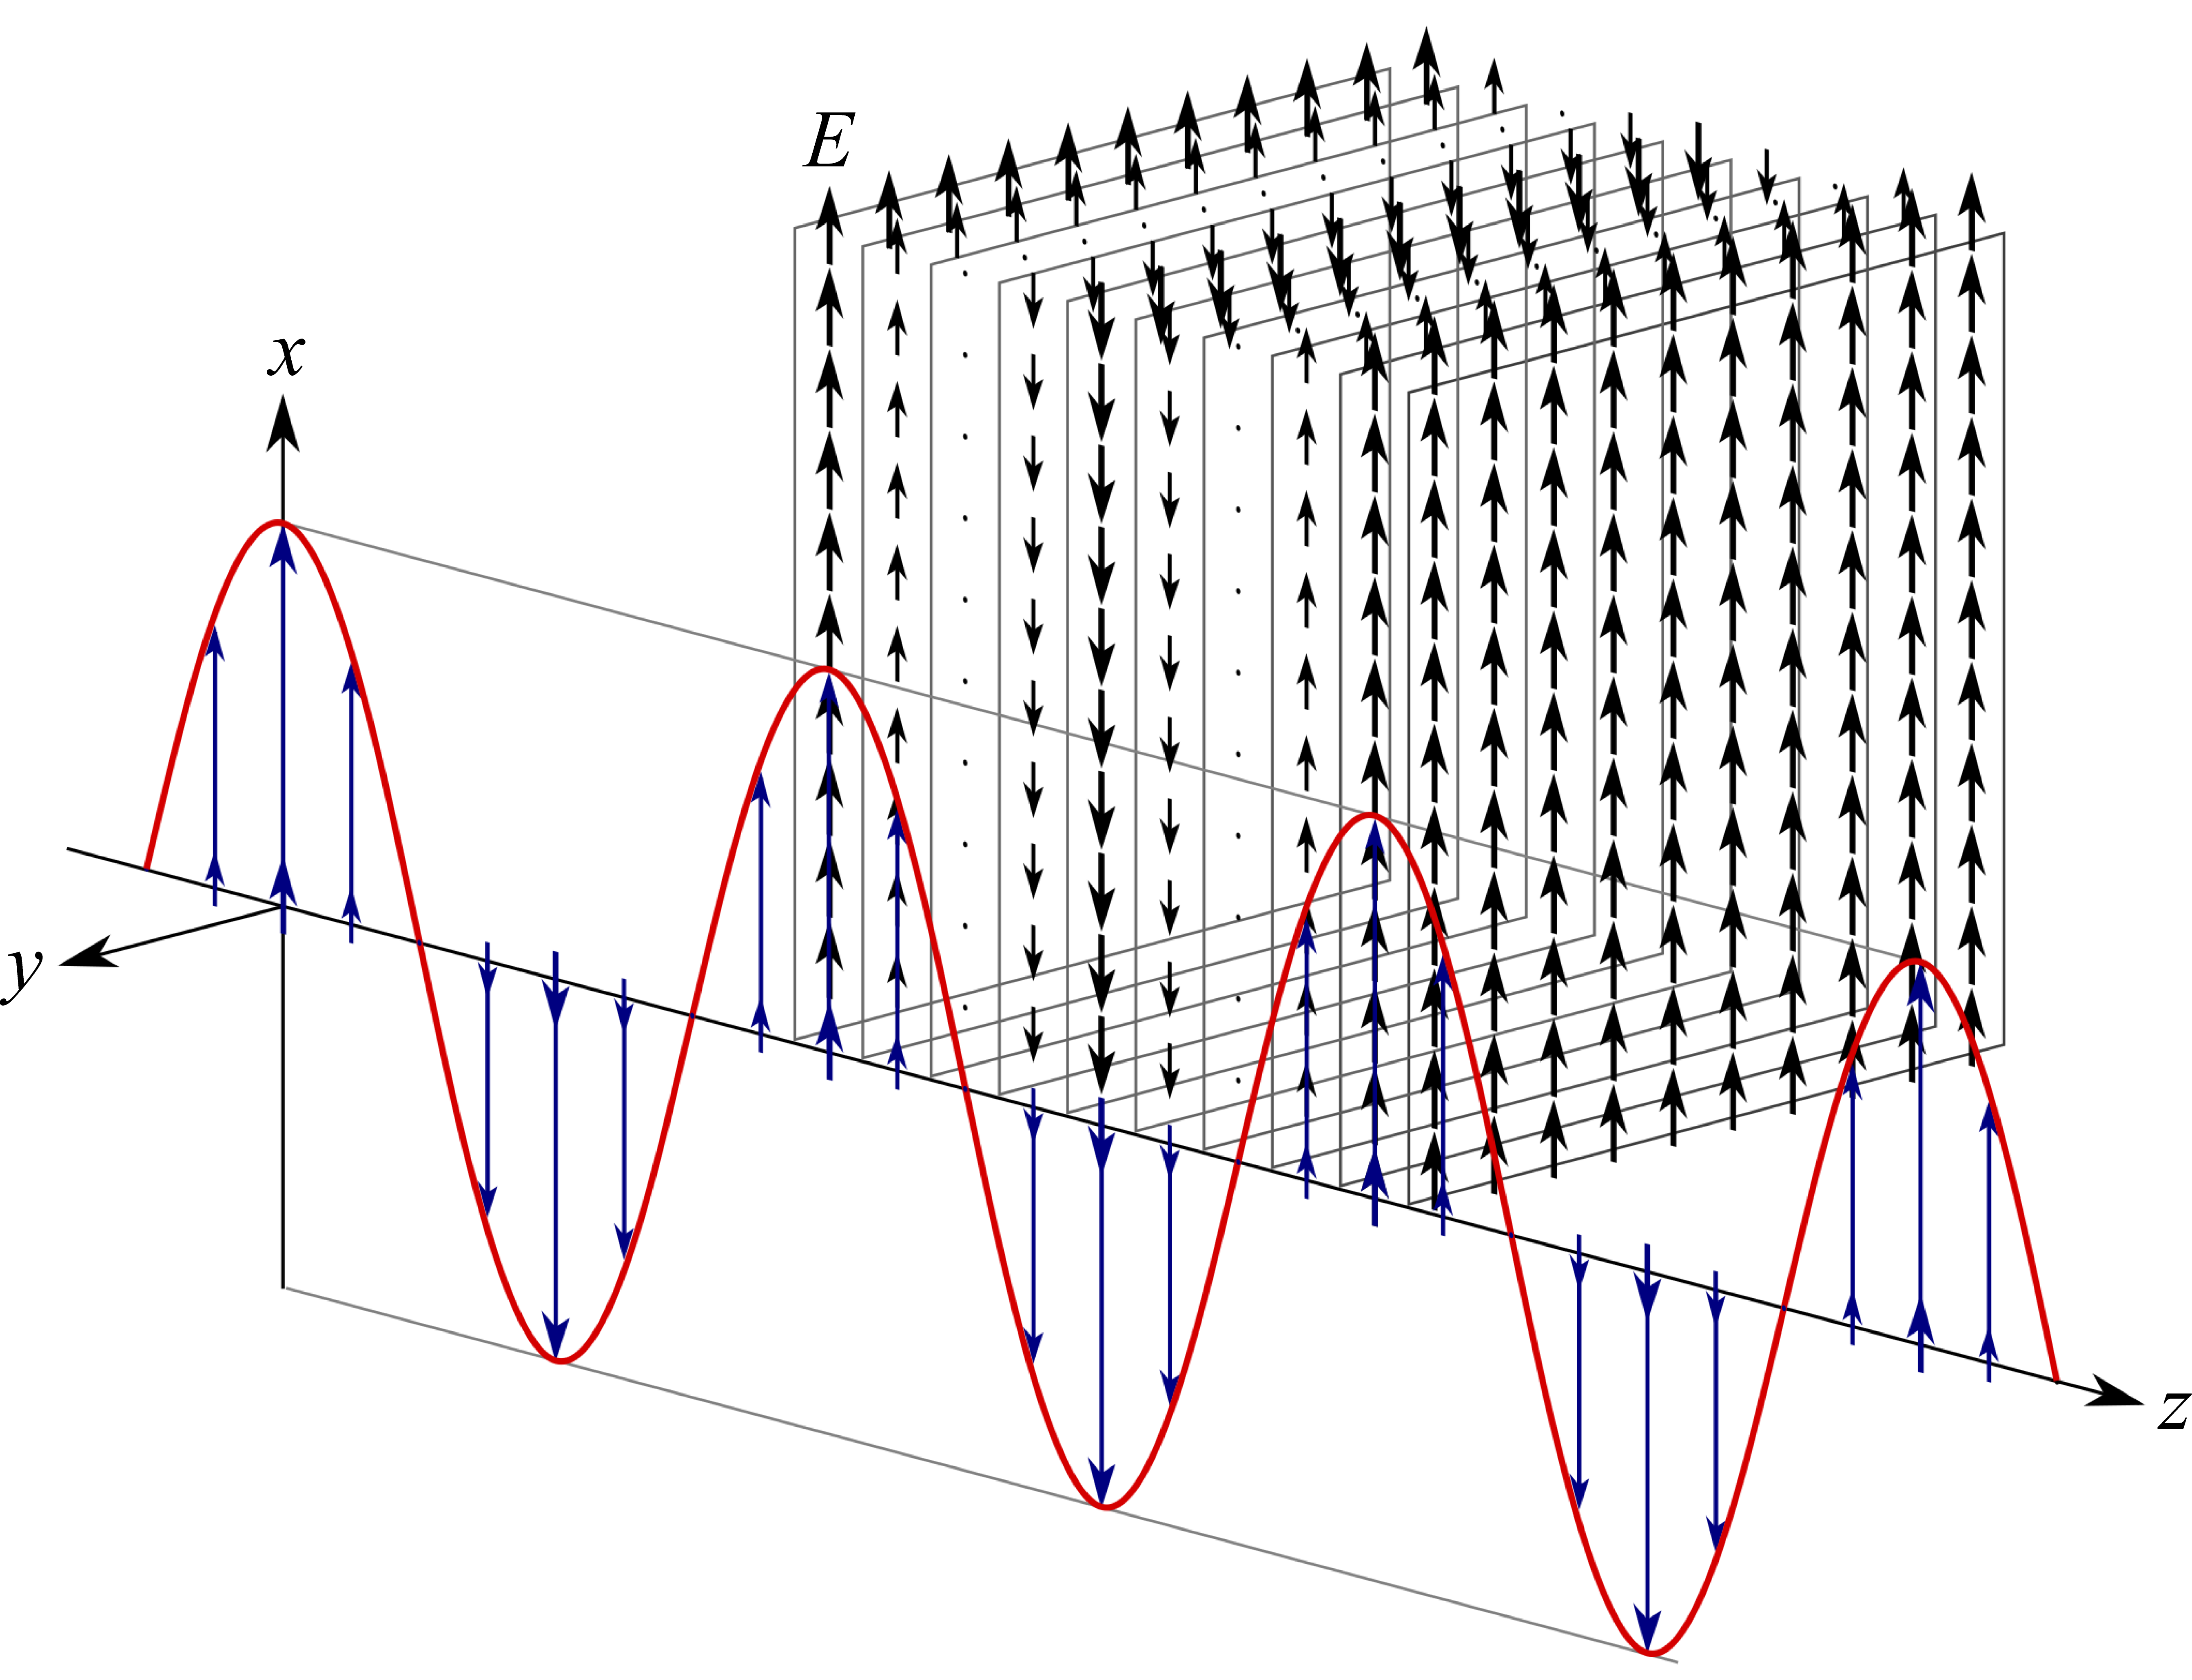
\includegraphics[width=8cm]{image/5-6-2.png}
\caption{平面偏振电磁波}
\end{wrapfigure}
光的波动理论建立在众多干涉衍射实验上,\,由19世纪后半页麦克斯韦({\it Maxwell}),\,韦伯({\it Weber})与赫兹({\it Hertz})等人的理论与实验工作进行总结与升华.\,最后通过迈克尔孙({\it Michelson})的干涉实验和随之由爱因斯坦({\it Einstein}),\,洛伦兹({\it Lorentz})等人建立的狭义相对论来完善与归入到更加普适的经典电磁场论下.\,然而整个18世纪实际上都处于光的粒子学说与波动学说的无休止争论中.\,这是因为此时发现的光的几乎所有现象都可以同时用两种学说进行解释.\,今天我们知道了光实际上也有\emph{波粒二象性}(particle-wave duality),\,最准确的描述光的语言应该是\emph{量子电动力学}(quantum electrodynamics,\,QED).\,光是一份份的量子场,\,被称为\emph{光子}(photon).\,几何光学问题,\,用经典的电磁场模型给出的描述最为精确,\,而在特殊场合或者精度要求不高的情况下,\,粒子光学的处理也是十分合适的.

真空中的\emph{平面波}(plane wave)提供了一种最为简单的情形,\,如图,\,此时$\bs{E}=E\bs{e}_x\cos(\omega t-kz)$.\,按照光学惯例,\,我们把它写作一个复数,\,模就是在每一点处场强的振幅,\,而幅角我们取为$\cos$里的相位宗量的相反数,\,而它的实部表示物理上的场强:
\[A(z,t)=E\ue^{\ui(kz-\omega t)}\]

有几点值得注意:\,首先,\,之所以取相反数,\,是因为在频率甚高的光频波段我们不太用关心每一个时空点处场随时间$t$的变化,\,而是不同时空点$z$对振幅与相位的影响,\,故把$kz$项提前.\,而对于$\omega t$项由于每一点的振动都含这个随时间振动的因子,\,而且角频率都是$\omega$(单色波),\,所以我们往往又省去这个因子写成$A=E\ue^{\ui kz}$,\,相当于仅考虑$t=0$时的初相位与振幅.\,这种操作意味着指数上的宗量随时间减小,\,这与我们平时对相位随时间增加的理解是相反的.\,其次,\,我们取消了其矢量性,\,我们知道沿特定方向$z$传播的平面单色电磁波可以分解为$x$方向的偏振与$y$方向的偏振,\,两者的同相反相组合可以造成不同方向的\emph{线偏振模式}(linear polarized mode),\,而相差$\dfrac{\pi}{2}$的组合则可以造成不同的\emph{圆偏振模式}(circular polarized mode).\,但这些只有在特殊的光学器件下进行偏振光干涉实验才能发现区别,\,故在一般的几何光学条件下我们只关心光的传播方向,\,相位与振幅信息,\,而不关心其偏振时用标量$A$来代表任意模式下约化的光的振幅大小,\,$A$具有电场强度的量纲\footnote{这是因为与物质发生相互作用而感光时电场的作用占据主导地位.},\,相同的$A$代表相同的光强与能流.\,$A$被称为\emph{标量振幅}(scalar amplitude).

平面波是其他一大类波在局部可以采取的近似,\,我们把等相位的面在局部近似为平面,\,则波传播方向为垂直于平面的法线方向,\,用\emph{波矢}(wave vector)$\bs{k}$代表这个方向,\,它的大小就是上述平面波的$k$,\,代表单位长度所改变的相位大小,\,正如\emph{角频率}(angular frequency)代表单位时间所改变的相位大小.\,两者具有如下关系:
\[\frac{\omega}{k}=\frac{\nu}{\sigma}=\frac{\lambda}{T}=\frac{c}{n}\]

其中$\nu$表示\emph{频率}(frequency),\,单位时间所经历的振动周期数,\,由于一个周期相位改变$2\pi$,\,故$\omega=2\pi \nu=\dfrac{2\pi}{T}$,\,同理,\,$\sigma$表示\emph{波数}(wave number),\,有$k=2\pi \sigma=\dfrac{2\pi}{\lambda}$,\,$\lambda$表示\emph{波长}(wave length)而$T$表示\emph{周期}(period).\,这里考虑到介质中的传播,\,波速小于真空中的波速,\,$n$为介质的\emph{折射率}(index of refraction).

而我们所要研究的更加普遍的一类光波一般写为:
\[A(\bs{r})=E(\bs{r})\ue^{\ui \varphi(\bs{r})}\]

这类光波的共性是仍然以统一地角频率$\omega$振动,\,也就是所谓的\emph{单色波}(monochromatic wave)\footnote{此时波的波动方程变为亥姆霍兹方程:\[\left[\nabla^2-\frac{1}{(c/n)^2}\frac{\partial^2}{\partial t^2}\right]A\ue^{-\ui \omega t}=0 \quad \Rightarrow \quad (\nabla^2+k^2)A=0\]}.\,所以我们省去包含时间的因子$\ue^{-\ui \omega t}$,\,直接写出只依赖于位矢$\bs{r}$的波动形式.\,一般来说$E$是$\bs{r}$的缓变函数,\,而$\varphi$则是$\bs{r}$的快速变化函数,\,且其变化要与波矢大小$k=\omega/c$相吻合:
\[\nabla \varphi=\bs{k}\]

例如,\,波源在$\bs{r}=0$的\emph{球面波}(spherical wave)有$E=\dfrac{u}{r},\,\varphi=kr$,\,而波源在$\rho=0$的\emph{柱面波}(cylindrical wave)有$\displaystyle E=\frac{u}{\sqrt{\rho}},\,\varphi=k\rho$.

\begin{figure}[H]
\centering
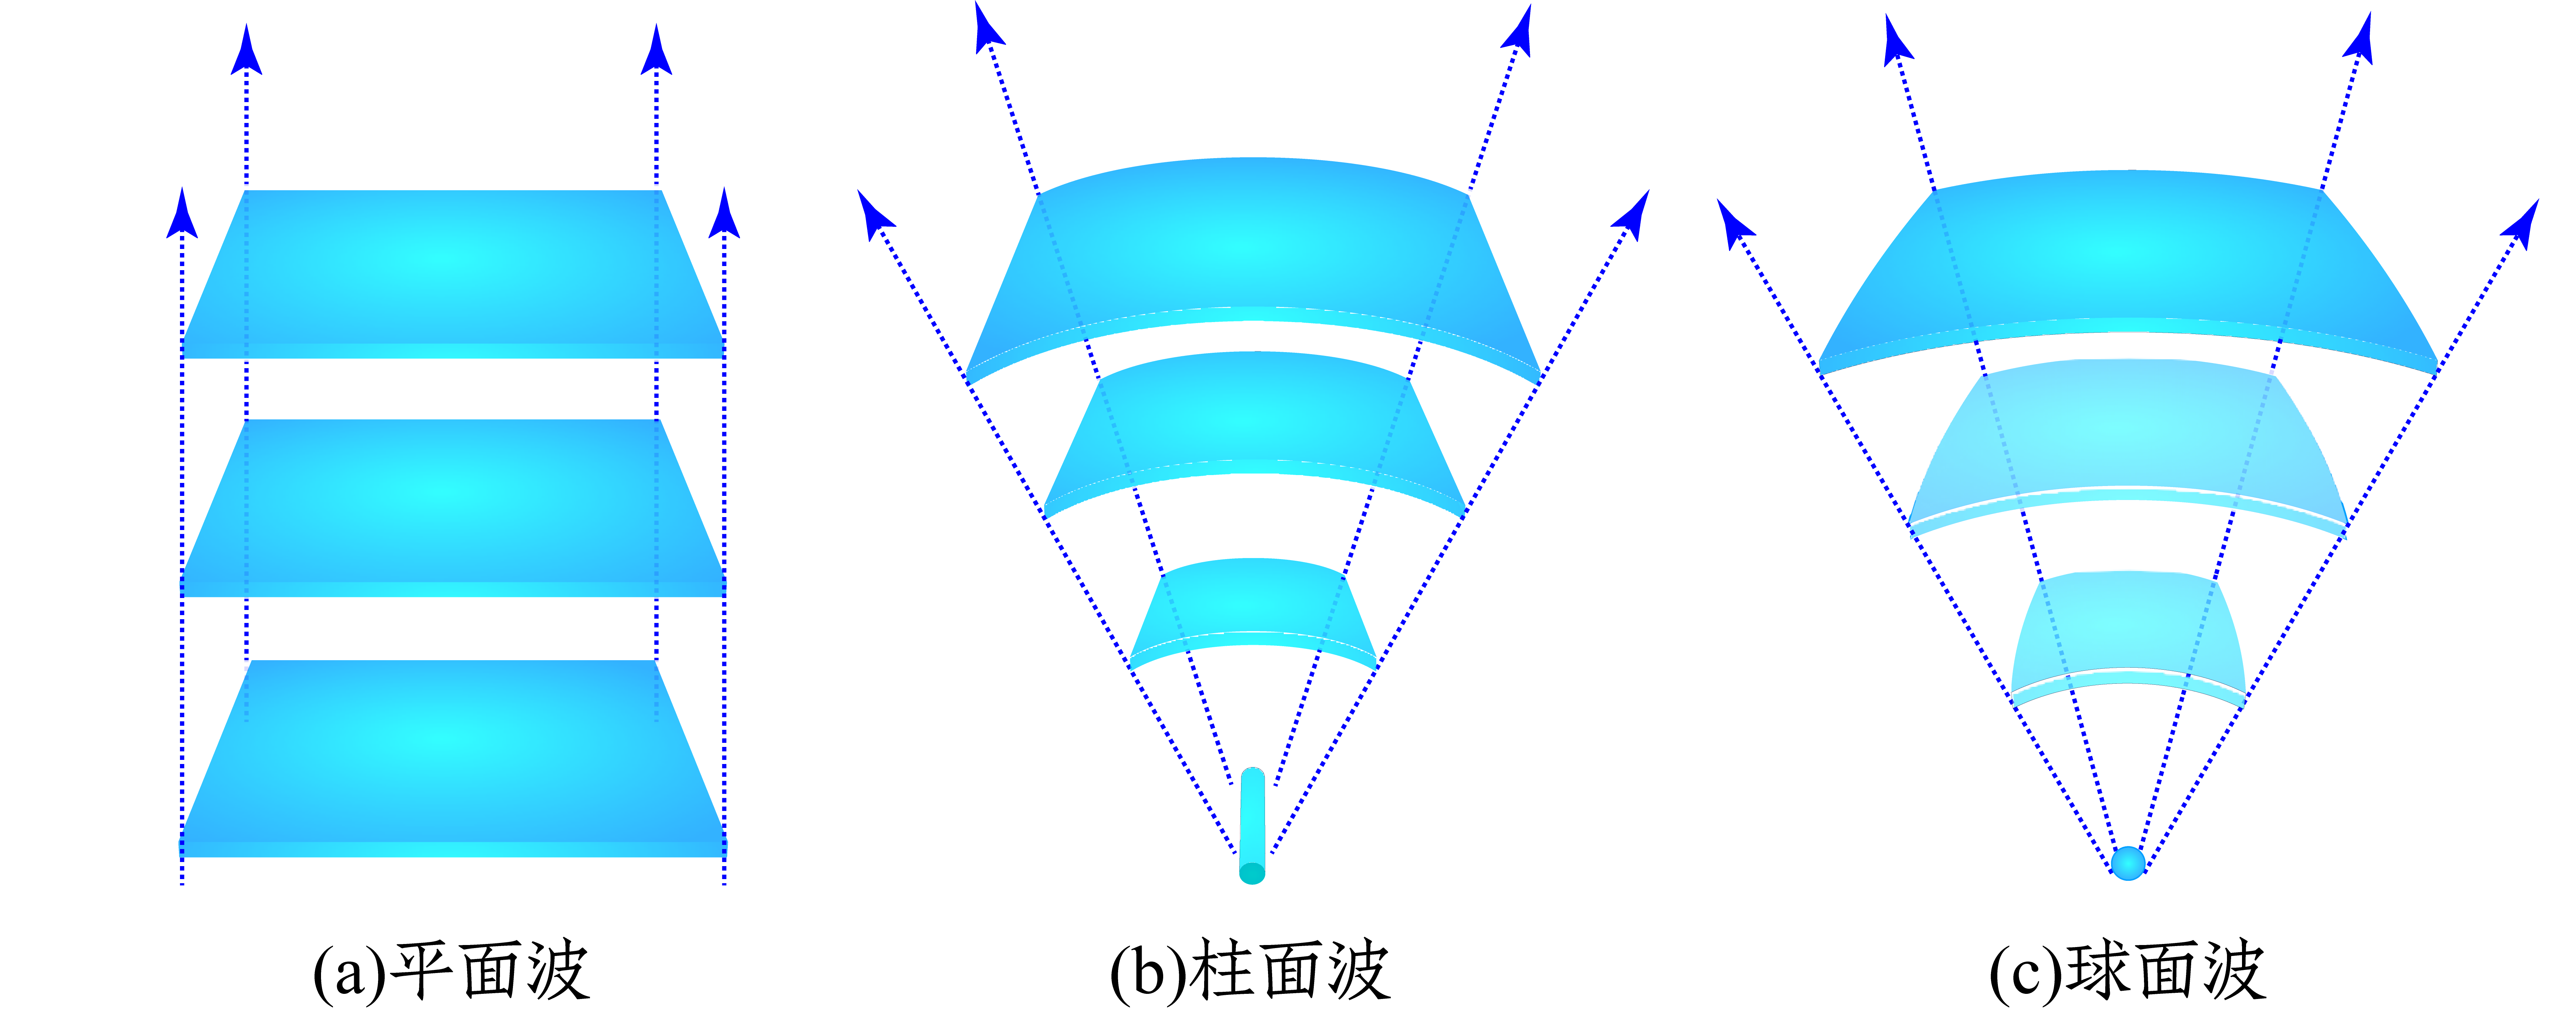
\includegraphics[width=0.8\textwidth]{image/5-6-3.png}
\caption{三种常用波形式}
\end{figure}

显然这些理想的波不能看成是生活中的一般光源的波特性,\,一言以蔽之,\,日常光波具有很差的\emph{相干性}(coherency).\,来自不同位置的点光源的不同偏振,\,不同频率,\,不同持续时间的波列非相关叠加,\,使得需要在十分仔细的实验条件下才可以观察到干涉衍射等现象.\,但这些对一般的几何光学性质没有影响,\,几何光学关心光的传播与光的强度,\,于是抽象出所谓的\emph{光线}(ray)的概念,\,光线$L$始终沿着波传播的方向,\,与等相位面垂直:
\[L:\quad \ud \bs{l}//\bs{k}=\nabla \varphi\]

对于以上理想的波光线的方向是显而易见的(图中虚线方向),\,而\emph{强度}(intensity),\,可以定义为$I=A^2$平面波不变,\,柱面波与半径成反比,\,球面波则与半径的平方成反比.\,而日常生活中的线状点状光源其性质在几何光学意义下是完全相同的.\,我们也可以把光的传播视为光线的集合,\,如果遇到界面则会发生折射与反射,\,折射率的不均匀导致光线的偏折,\,而波前可以被部分的障碍物遮挡,\,没被遮挡的部分仍然以光线的方式向前传播.

也就是说,\,在几何光学研究中,\,光线是表,\,其实作为电磁场的光波才是里.\,光在两种介质表面的\emph{反射}(reflection)与\emph{折射}(refraction)就是波动理论应用的绝佳例证.

\subsection{菲涅尔公式}

\begin{wrapfigure}[10]{o}[-10pt]{7cm}
\centering
\vspace{-2cm}
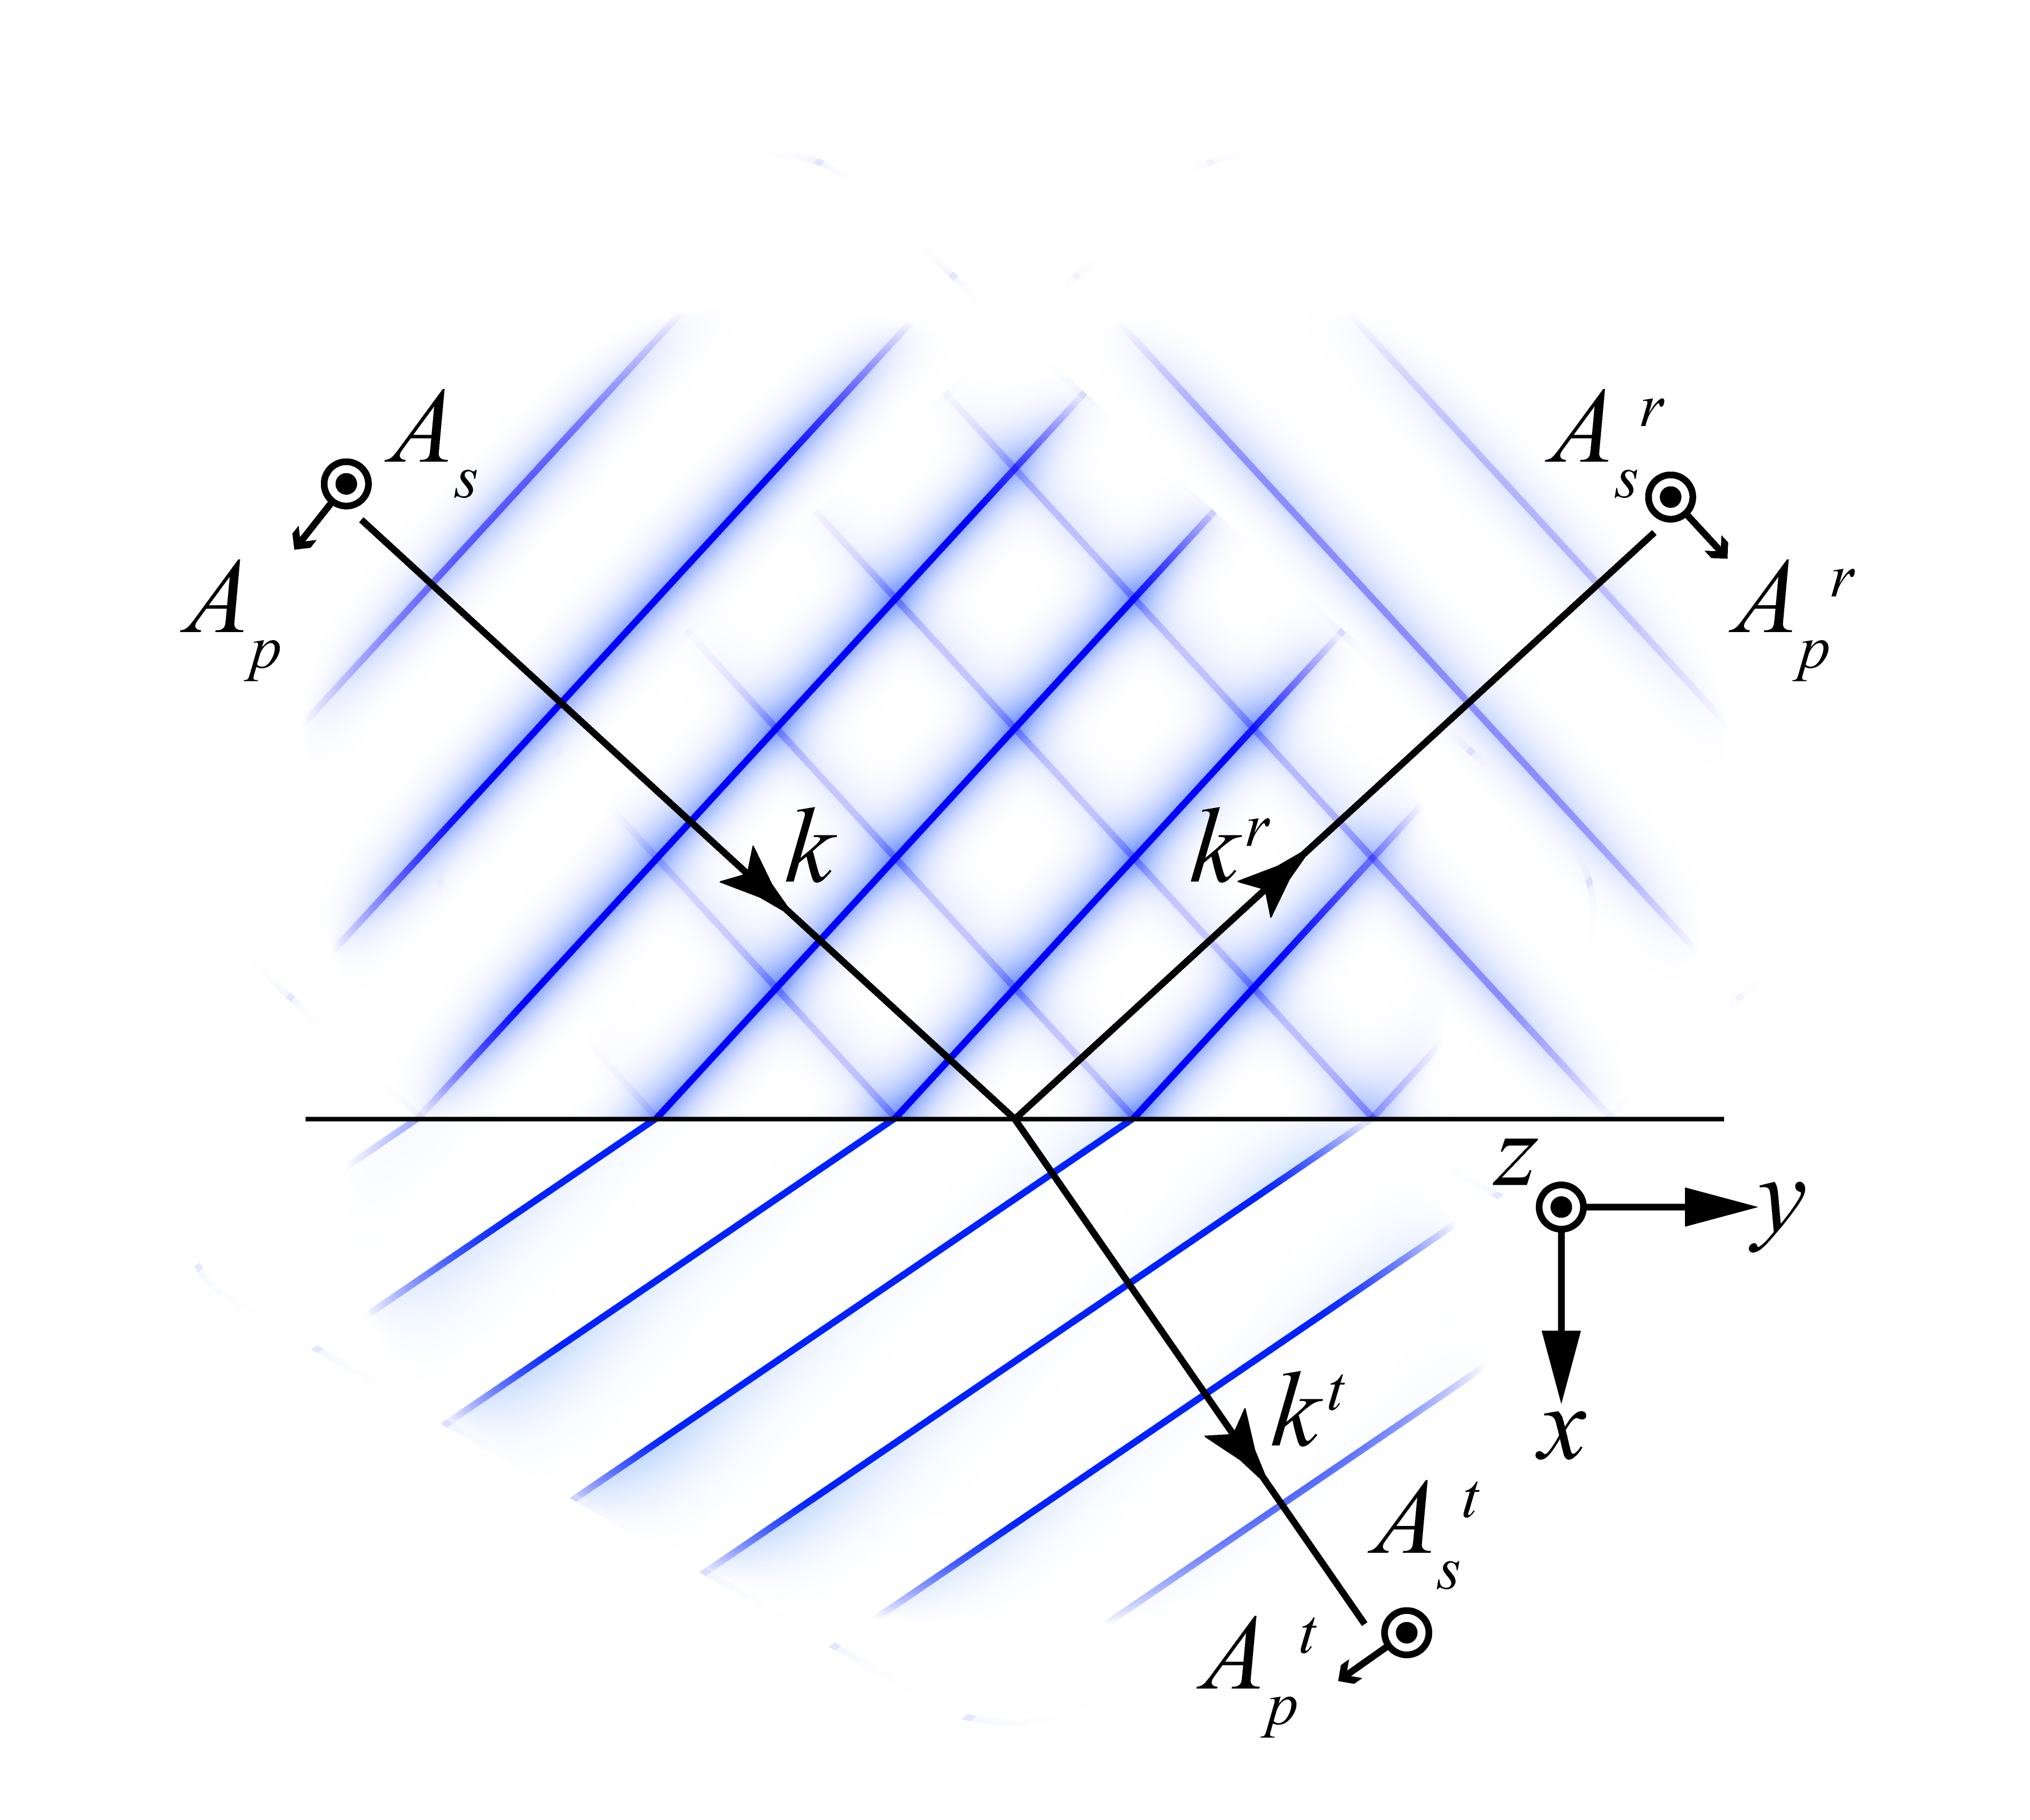
\includegraphics[width=8cm]{image/5-6-4.png}
\caption{界面与两种模式}
\end{wrapfigure}
如图,\,在一个典型的界面上反射与折射的过程中,\,反射光,\,折射光的强度实际上是与入射光的偏振状态有关的.\,这一点在接下来的计算中也可以表明.\,我们按照惯例,\,取两个独立的线偏振为:
\begin{itemize}
	\item \emph{横电波}(TE wave),\,即垂直偏振波(s\footnote{来自德语词senkrecht:\,垂直.}-wave,\,s-polarized wave),\,它的电场方向垂直于主平面\footnote{由入射线与界面法线确定的平面,\,显然,\,出射波与折射波光线方向也在这个平面内.}.\,而磁场方向则在主平面内.
	\item \emph{横磁波}(TM wave),\,即平行偏振波(p\footnote{来自德语(英语)词parallel:\,平行.}-wave,\,p-polarized wave),\,它的电场方向平行与主平面.\,而磁场方向垂直主平面.
\end{itemize}

\npg{-3cm}

它们的正方向如图所示,\,满足\(\bs{A}_s\times\bs{A}_p//\bs{k}\).\,而反射折射系数则定义为在\((0,0,0)\)点处的界面两侧各光振幅比:
\[A_{s,p}=E_{s,p}\ue^{\ui(\bs{k}\cdot \bs{r}-\omega t)}\; ,\; A_{s,p}^r=E_{s,p}^r \ue^{\ui(\bs{k}^r \cdot \bs{r}-\omega^r t)}\; ,\; A_{s,p}^t=E_{s,p}^t \ue^{\ui(\bs{k}^t \cdot \bs{r}-\omega^t t)}\]
\[r_{s,p}=\frac{E_{s,p}^r}{E_{s,p}}\; ,\; t_{s,p}=\frac{E_{s,p}^t}{E_{s,p}}\]

对于$s$-光,\,电磁场在界面两侧切向电场连续,\,切向磁场强度连续\footnote{法向电位移为零.}.\,而对于$p$-光,\,切向也有电场连续,\,法向可以用电位移连续.\,注意到边界条件对任意$t$成立,\,这给出了:
\[\omega=\omega^r=\omega^t\]

也就是折射反射不能改变光的频率,\,也就是颜色.\,从光量子论的角度理解这代表\emph{弹性}(elastic)作用,\,光子的能量将不受改变,\,介质不会以某种共振的方式吸收入射光的能量.\,上式还意味着\(k=\dfrac{\omega}{c/n}=n\dfrac{\omega}{c}=nk_0\propto n\),\,介质内的波矢比同样颜色的真空光要大折射率$n$倍.

而这个边界条件对任意界面$y$坐标也是恒成立的,\,这给出了:
\[k_y=k\sin\theta=k^r\sin\theta^r=k^t\sin\theta^t\]

即折射时平行于界面方向的波矢是不变的.\,光量子论下可以理解为这个方向动量不变,\,没有受到沿平行界面方向的相互作用.\,但注意到$k$与$n$的正比关系,\,将折射方折射率记做$n'$,\,折射角记做$\theta'$我们得到了著名的\emph{斯涅耳定律}(Snell's Law):
\[\theta^r=\theta \quad ;\quad n\sin\theta=n'\sin\theta'\]

再注意到在光学问题中我们一般只讨论透明介质,\,它们磁导率十分接近真空\(\mu\approx \mu_0\),\,在此时实际上\(\dfrac{c}{n}=\dfrac{1}{\sqrt{\varepsilon\mu}}\)给出了\(n=\sqrt{\dfrac{\varepsilon}{\varepsilon_0}}=\sqrt{\varepsilon_r}\).\,而此时实际上电位移振幅就是\(D=\varepsilon E=n^2\varepsilon_0 E\propto n^2 E\)磁感应强度振幅就是\(B=\sqrt{\varepsilon\mu}E=\dfrac{n}{c}E\propto nE\),\,磁场强度$H$与它只差一个真空磁导率$\mu_0$.\,依此我们写出$s$-光与$p$-光的边界条件:
\[E_s+E_s^r=E_s^t\quad ;\quad nE_s\cos\theta-nE_s^r\cos\theta=n'E_s^t\cos\theta'\]
\[E_p\cos\theta-E_p^r\cos\theta=E_p^t\cos\theta'\quad ;\quad n^2E_p\sin\theta+n^2E_p^r\sin\theta=n'^2E_p^t\sin\theta'\]

解之,\,我们得到的则是著名的\emph{菲涅尔公式}(Fresnel's equations):
\[r_s=\frac{n\cos\theta-n'\cos\theta'}{n\cos\theta+n'\cos\theta'}\quad ;\quad t_s=\frac{2n\cos\theta}{n\cos\theta+n'\cos\theta'}\quad ;\quad t_s-r_s=1\]
\[r_p=\frac{n'\cos\theta-n\cos\theta'}{n'\cos\theta+n\cos\theta'}\quad ;\quad t_p=\frac{2n\cos\theta}{n'\cos\theta+n\cos\theta'}\quad ;\quad \frac{n'}{n}t_p-r_p=1\]

都满足:
\[n(1-|r_{s,p}|^2)\cos\theta=n'|t_{s,p}|^2\cos\theta'\]

其中\emph{反射率}(reflectance)与\emph{透射率}(transmittance)分别被定义为:
\[R_{s,p}=|r_{s,p}|^2\quad;\quad T_{s,p}=\frac{n'\cos\theta'}{n\cos\theta}|t_{s,p}|^2\]

透射率与透射振幅系数\(t_{s,p}\)关系前多出来的系数,\,一是由于在介质中能流密度正比于折射率\(I\propto |\bs{E}\times\bs{H}|\propto nE^2\),\,二是折射后方向改变,\,两侧对应光束部分的横截面积也会发生改变.\,下图展示了空气(\(n=1\))与玻璃(\(n=1.5\))界面上的\emph{外入射}(external incidention)与\emph{内入射}(internal incidention)时的情形.
\begin{figure}[H]
\centering
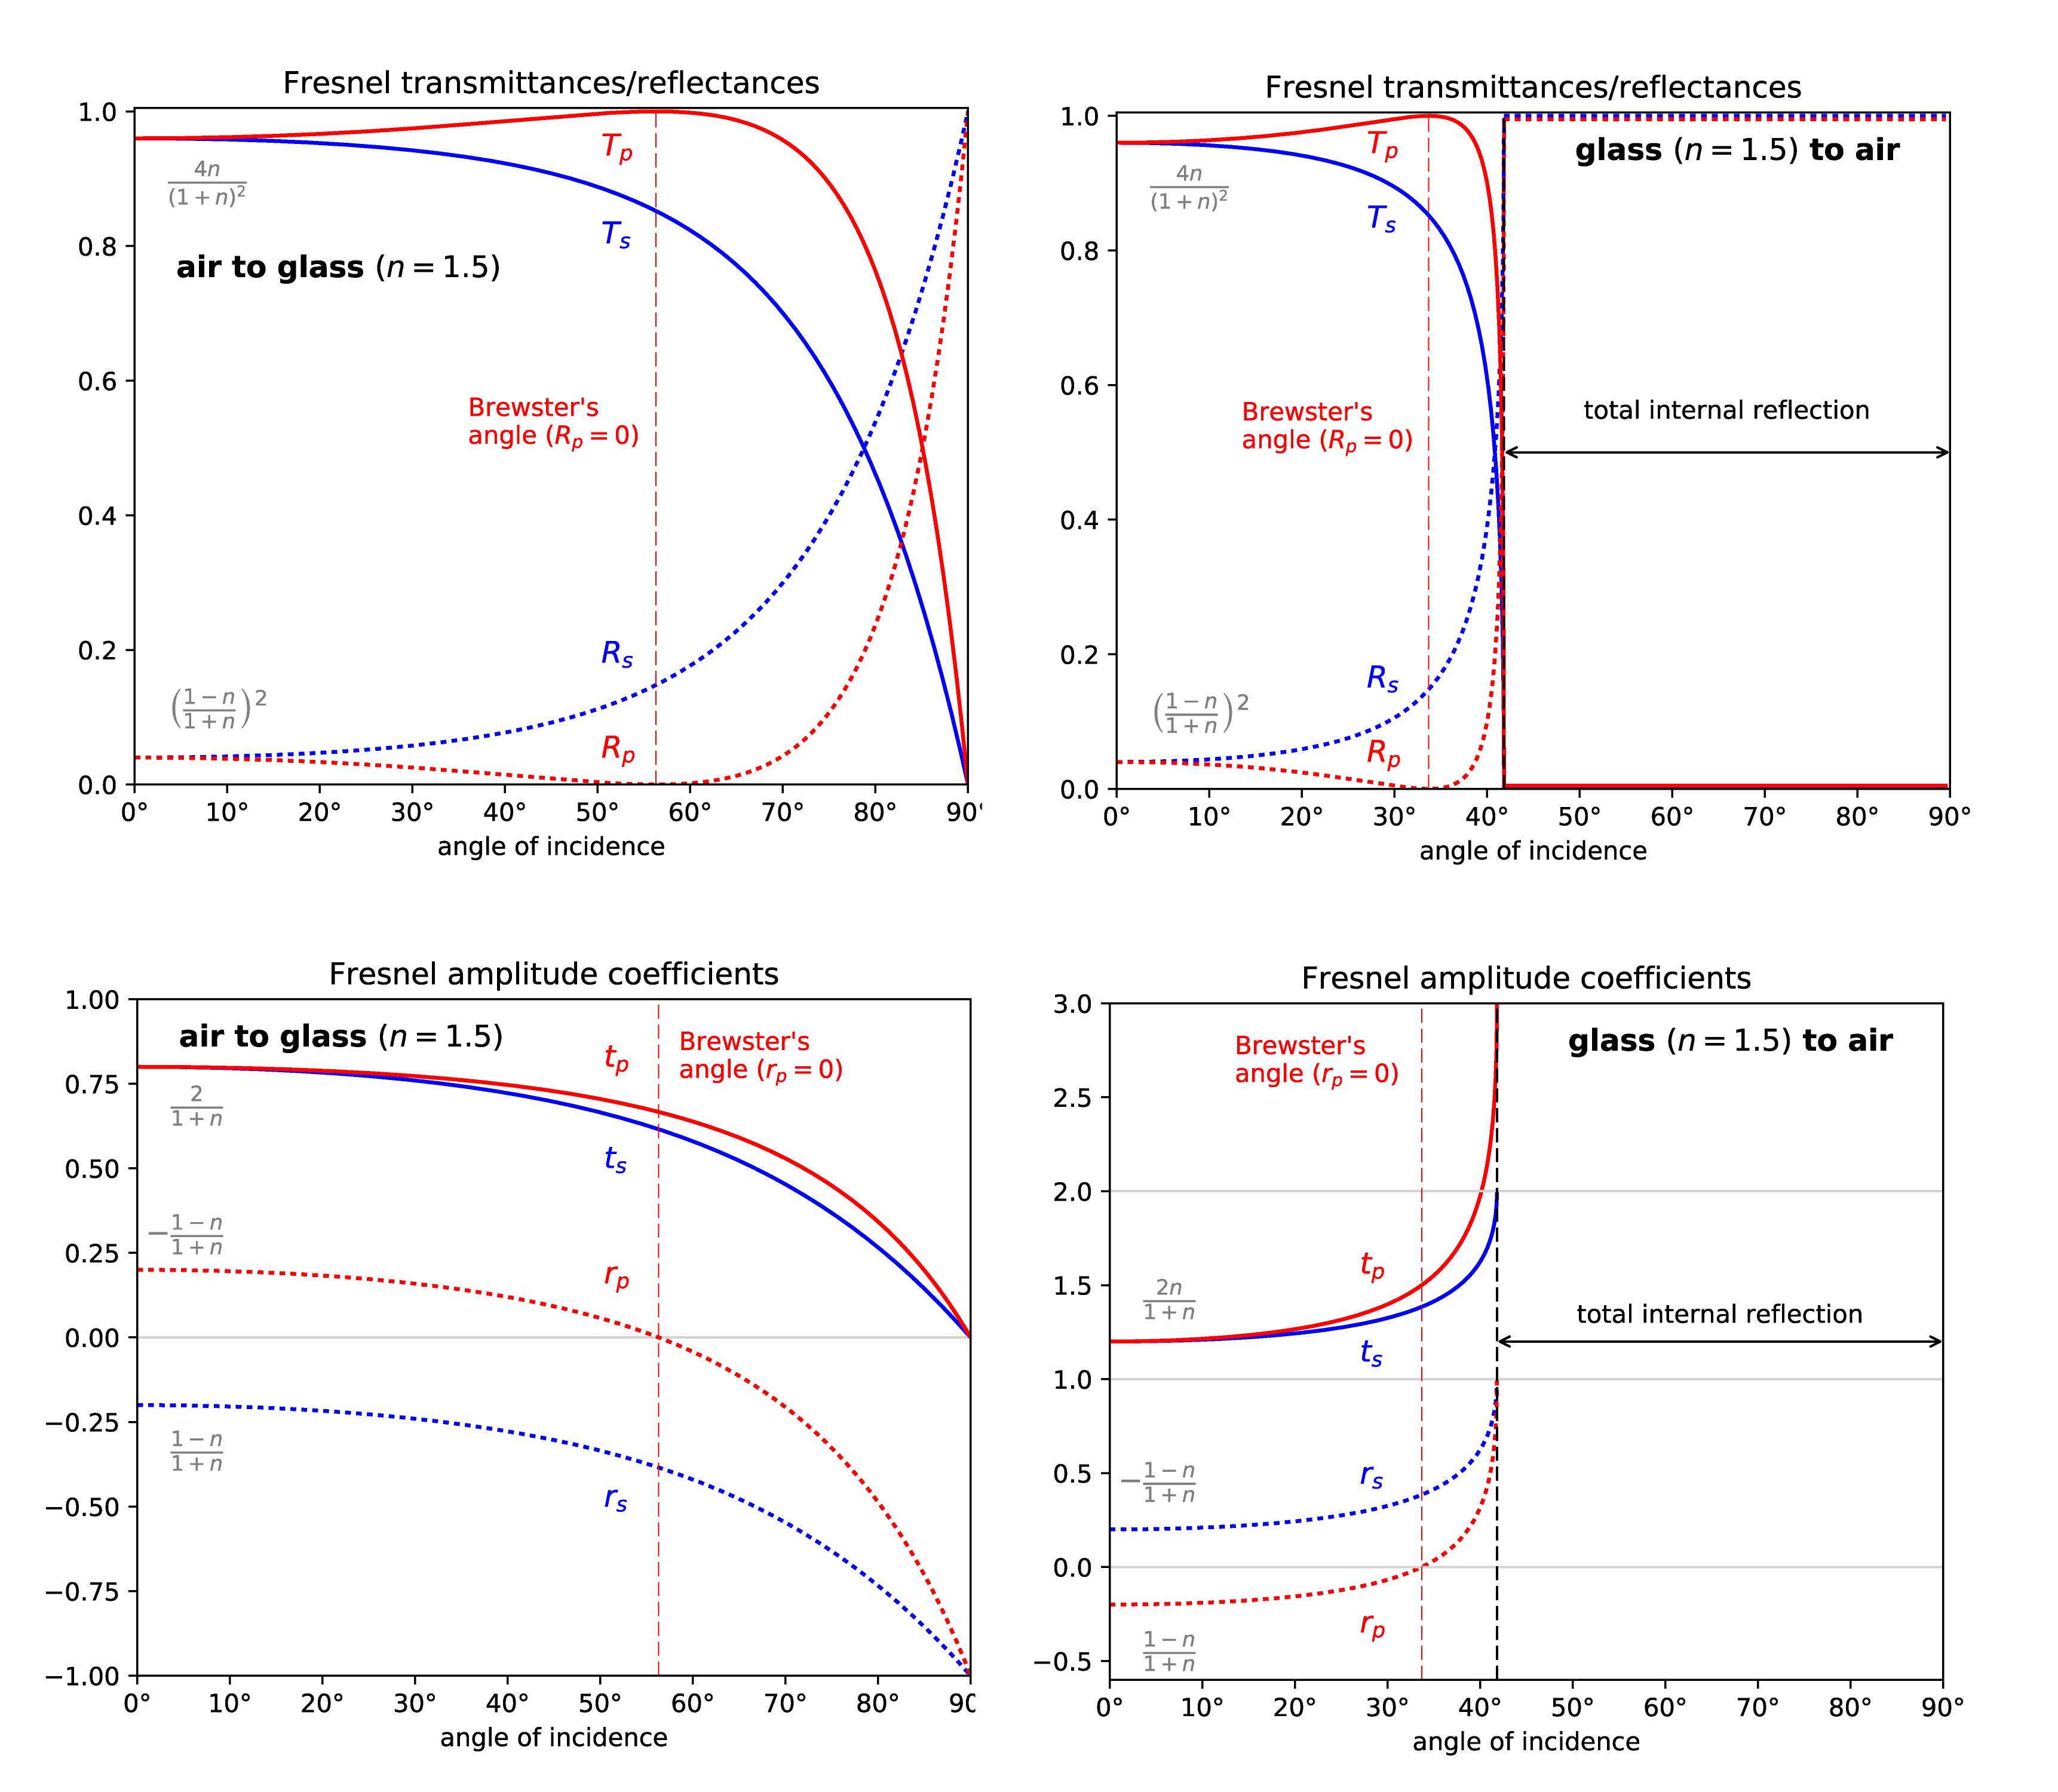
\includegraphics[width=0.8\textwidth]{image/5-6-5.png}
\caption{界面反射与折射}
\end{figure}

有几点值得注意:

\subsubsection{\hei 半波损失发生条件}

当正入射时,\,反射光可以与入射光发生叠加.\,我们关心在$x=0$处,\,也就是界面上的叠加结果.\,当$n'>n$时,\,由上图可见\(r_p>0\)而\(r_s<0\).\,但注意到在此处我们预设的入射反射电场正方向对$p$-光本来也相反而$s$-光相同.\,故事实上都是相干相消.\,发生了\emph{半波损失}(half-wave loss).\,而若$n'<n$时情况恰好相反,\,两种光都是相干相长,\,没有半波损失.

而对于入射角为\(90^\circ\)的掠入射情形,\,观察可知\(r_{s,p}=-1\),\,即反射光完全与入射光交叠区域几乎完全相干相消.\,这个结论对两种偏振模式与两种入射方式均给出了半波损失的结果.

注意透射光几乎在所有情形下都与入射光同相.\,唯一的例外发生在全内反射情况下.\,之后将仔细讨论之.

\subsubsection{\hei 布儒斯特角}

\begin{wrapfigure}[8]{o}[-10pt]{6cm}
\centering
\vspace{-2cm}
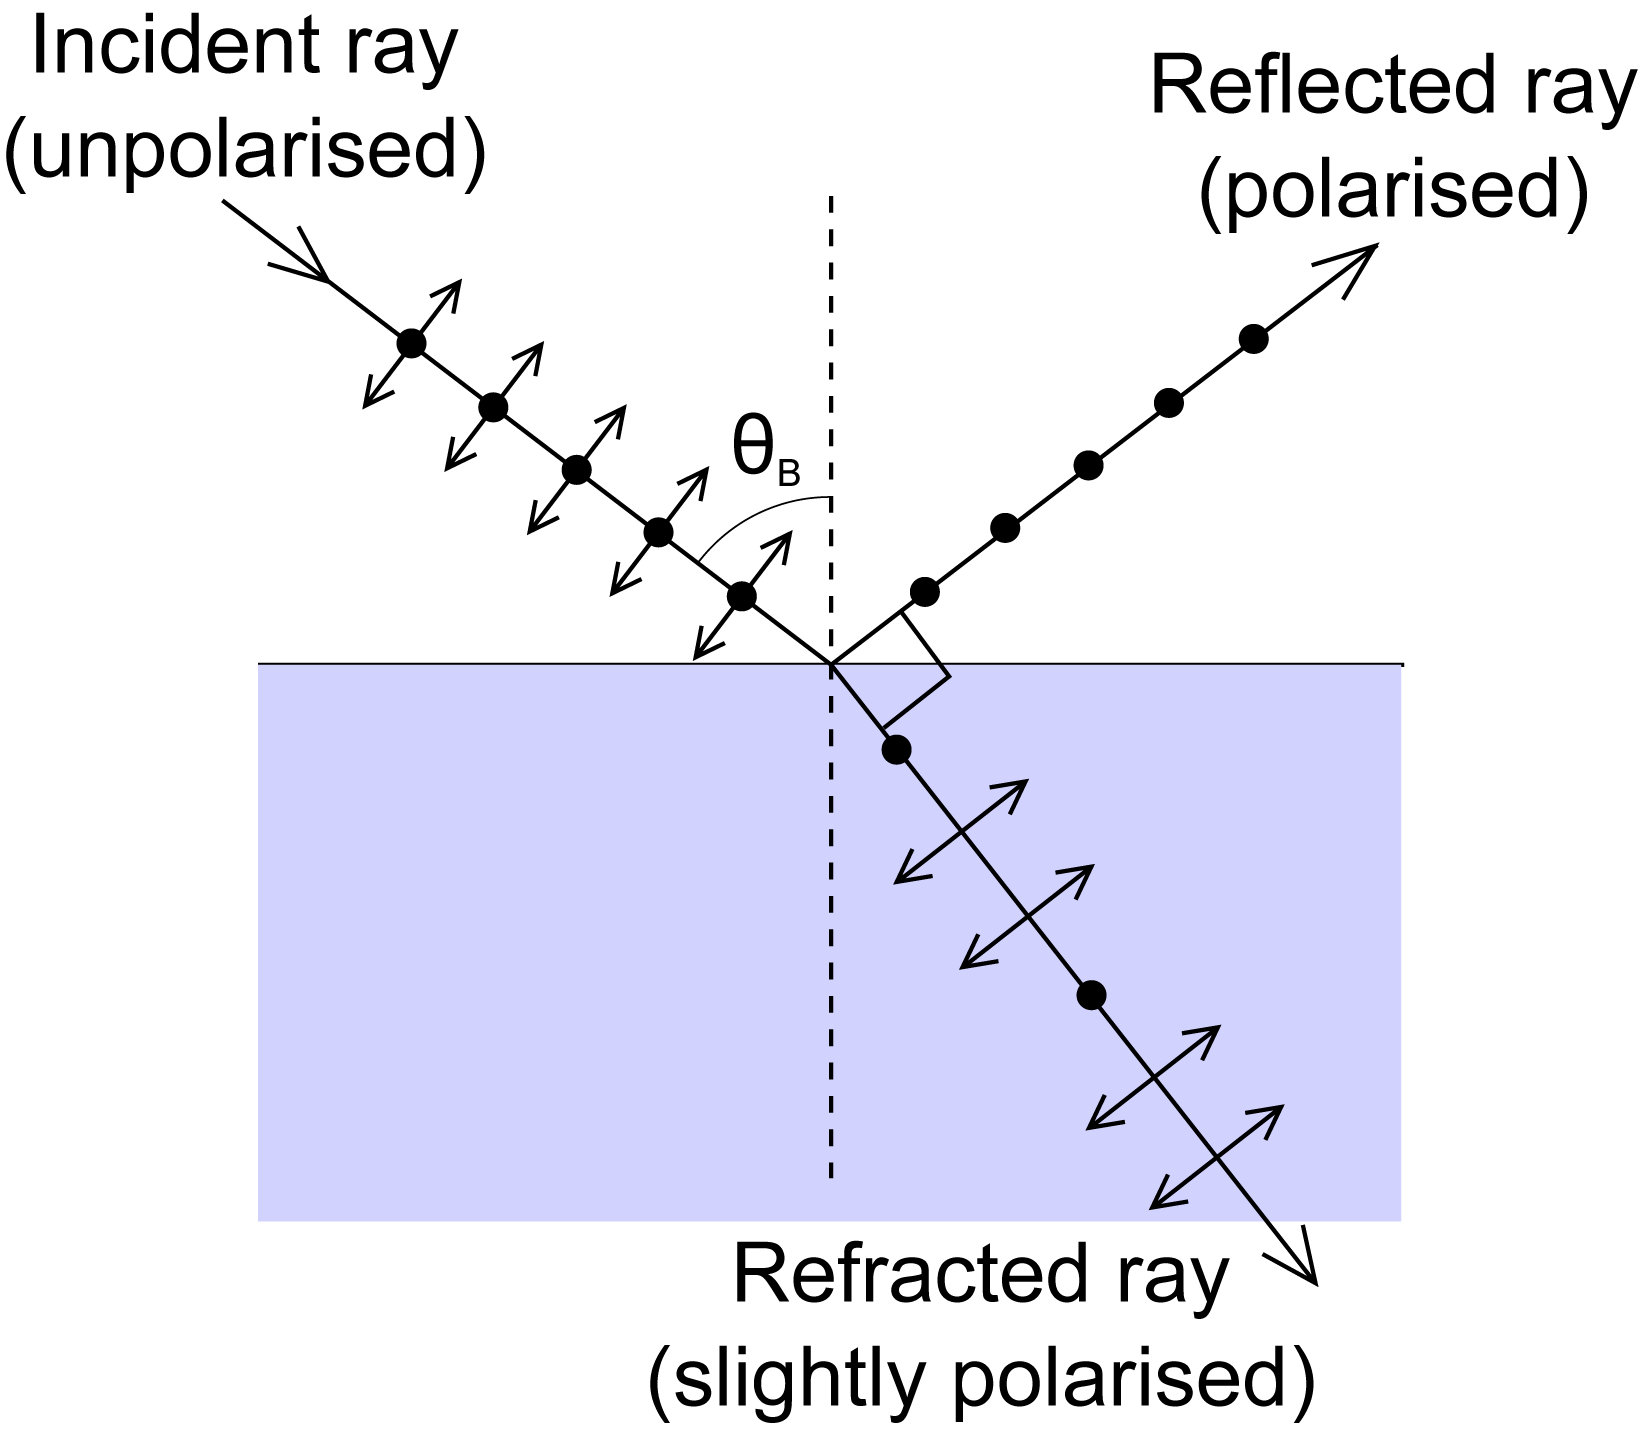
\includegraphics[width=6cm]{image/5-6-6.png}
\caption{布儒斯特角}
\end{wrapfigure}
注意到:
\[r_p=\frac{n'\cos\theta-n\cos\theta'}{n'\cos\theta+n\cos\theta'}=\frac{\sin\theta\cos\theta-\sin\theta'\cos\theta'}{\sin\theta\cos\theta+\sin\theta'\cos\theta'}=\frac{\tan(\theta-\theta')}{\tan(\theta+\theta')}\]

可以发现在\(\theta+\theta'=\dfrac{\pi}{2}\)时\(r_p=0\),\,横电的$p$-光将发生消光的情形.\,这种特殊的情况在内入射与外入射时都可以发生.\,对应的入射角称为\emph{布儒斯特角}(Brewster's angle).\,其原因可以这样理解:\,将入射波变为折射波与反射波实际上是介质电偶极子在电场驱动下振动的集体结果.\,而对于$p$-光,\,反射方向恰恰是介质内电场激发的偶极振动的振动方向.\,按照电磁波的辐射理论,\,这个方向上恰好是辐射强度为零的.\,所以恰好反射波消失.

依照这一种特性制作出来的\emph{布儒斯特窗}(Brewster window)常见于各种气体激光器的内置谐振腔或发射口.\,它将一块透明介质倾斜至布儒斯特角的位置,\,它有效地将$s$-光进行反射,\,而$p$-光没有反射的直接出射,\,使得出射激光一般都是沿p-方向高度偏振的.

\subsubsection{\hei 全内反射与隐失波}

在内入射状态下如果入射角足够大,\,根据斯涅耳定律将无法确定折射角\(\sin\theta'>1\).\,这种情形为\emph{全内反射}(total internal reflection).\,因为接下来的计算可以表明反射系数\(R_{s,p}=1\).\,而实际上此时并不是完全没有折射光场,\,而是折射光场被局域在有光照射的表面区域无法传播开来.

首先,\,折射光场由于边界条件在边界上每个时空点都成立,\,它依然符合:
\[\omega'=\omega\quad ,\,\quad k_y'=k_y=k\sin\theta\]

但此时由于\(x,y\)方向波矢仍然满足\(\displaystyle k_x'^2+k_y'^2=k'^2\),\,而由于入射角足够大使得\(k_y>k'\),\,所以实际上$k_x'$只能成为一个虚数:
\[k_x'=\pm\ui \kappa\quad ;\quad \kappa=\sqrt{k^2\sin^2\theta-k'^2}=\frac{\omega}{c}\sqrt{n^2\sin^2\theta-n'^2}\]

取正号还是取负号呢?\,这实际上取决于我们想研究的问题.\,在此处我们关心\(k_x=+\ui\kappa\)的解.\,这是因为这使得相位因子\(\displaystyle \ue^{\ui k_x x}\)成为衰减因子\(\displaystyle \ue^{- \kappa x}\)而不是正的指数爆炸因子\footnote{这意味着下方的场才是需要关心的而界面上的场仅仅是弱地可以忽略的边缘效应.}.\,这样,\,再将菲涅尔公式中的各个\(\cos\theta\)理解为\(\dfrac{k_x}{k}\),\,我们得到:
\[r_s=\ue^{-2\ui \delta_s}\; ,\; t_s=\frac{2n\cos\theta}{\sqrt{n^2-n'^2}}\ue^{-\ui\delta_s} \quad,\quad\delta_s=\arctan\frac{\sqrt{n^2\sin^2\theta-n'^2}}{n\cos\theta}\]
\[r_s=\ue^{-2\ui \delta_p}\; ,\; t_p=\frac{2nn'}{\sqrt{(n^2-n'^2)(n^2\tan^2\theta-n'^2)}}\ue^{-\ui\delta_p} \quad,\quad\delta_p=\arctan\frac{n\sqrt{n^2\sin^2\theta-n'^2}}{n'^2\cos\theta}\]

\vspace{0.5cm}
\begin{wrapfigure}[13]{o}[-10pt]{7cm}
\centering
\vspace{-1cm}
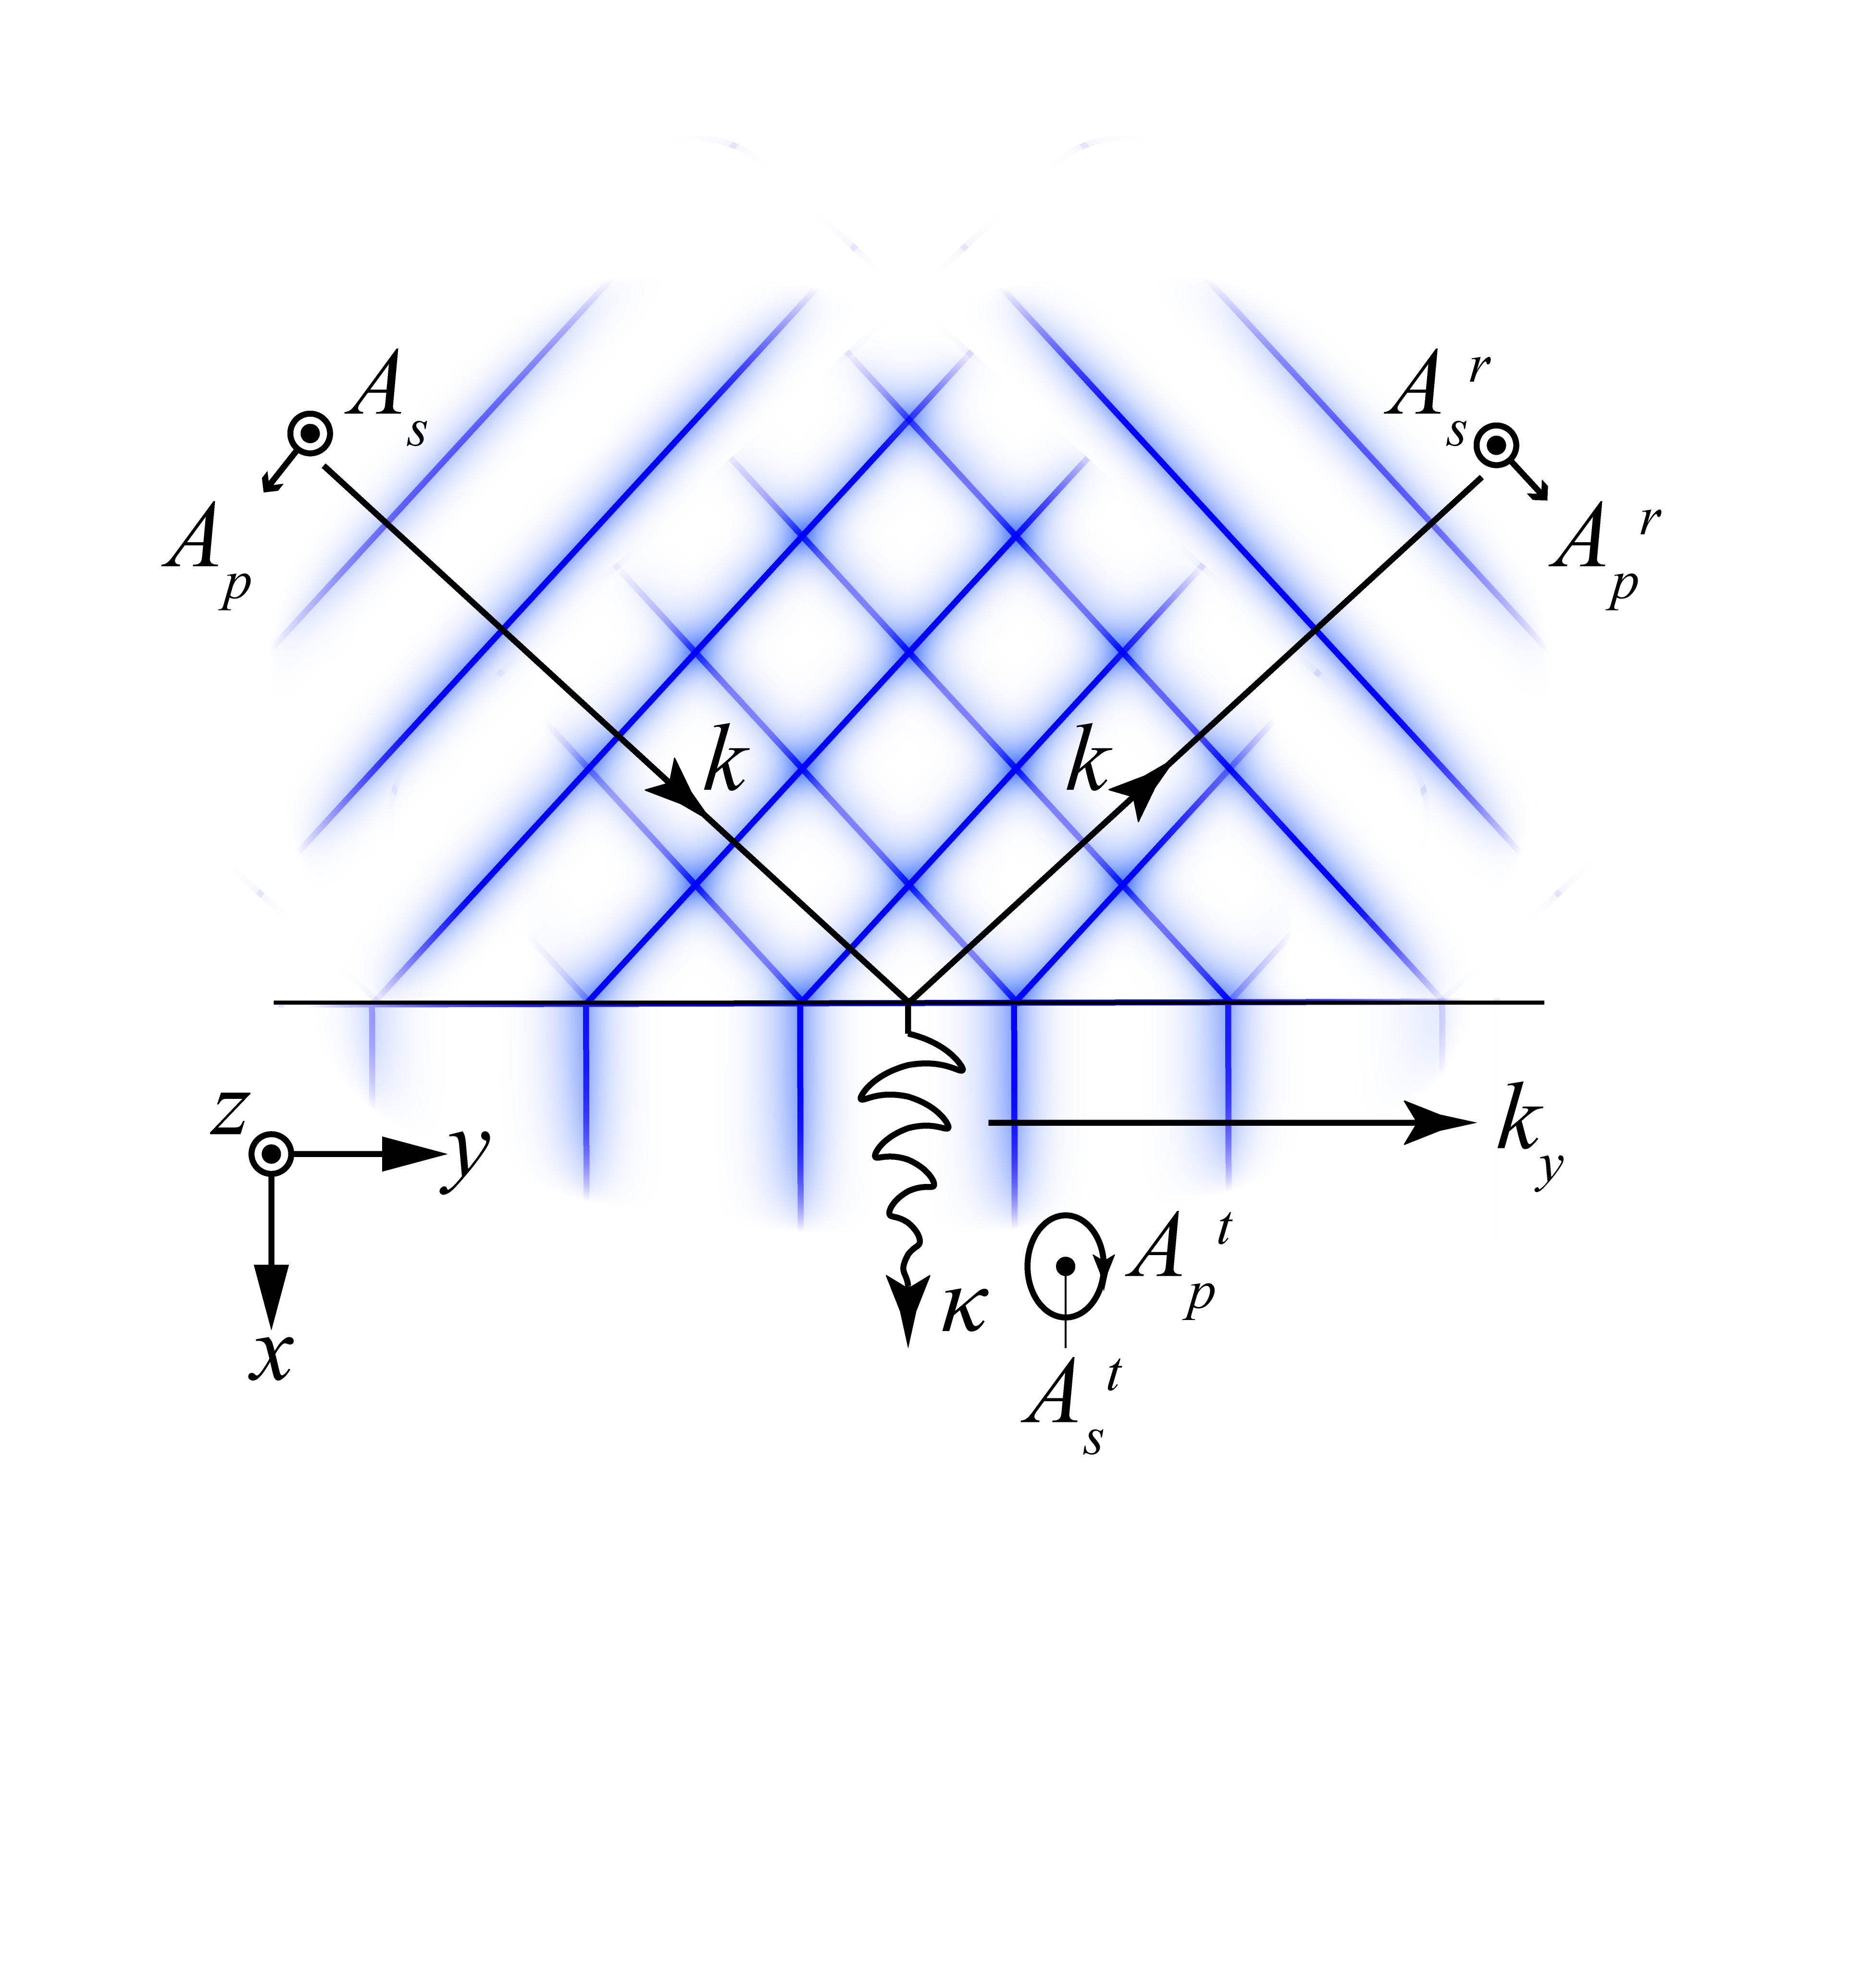
\includegraphics[width=8cm]{image/5-6-7.png}
\vspace{-3cm}
\caption{全内反射与隐失波}
\end{wrapfigure}
可见,\,此时最显著的特点除了反射振幅系数的模为一,\,就是反射波将会与入射波拉开一个非$0$非$\pi$的相位差\(2\delta_s\),\,它随着从临界全内反射到掠入射从$0$不断增加至$\pi$.\,而折射波相位则恰好介于两者之间,\,其振幅在临界全内反射时有极大值,\,此后随着入射角增加而不断减小至零.

更细致的分析可以发现折射光场的$p$-光模式实际上是$x-y$平面上的顺时针椭圆偏振光.\,$s$-光模式则显然还沿垂直平面的$z$方向.\,两者都要在$x$方向上做衰减,\,指数衰减可以表示为:
\[A(x)=A(0)\ue^{-\frac{x}{H}}\]

其中\(\displaystyle H=\frac{1}{\kappa}=\frac{\lambda_0}{2\pi\sqrt{n^2\sin^2\theta-n'^2}}\)称为\emph{衰减深度}(attenuation depth)或\emph{趋肤深度}(skin depth),\,\(\lambda_0\)是真空中的该色光波长.\,由表达式可见其一般$H$就光的波长的数量级.\,正是因为这个原因这种折射波被称为\emph{隐失波}(evanescent field).\,它一定会产生但是由于存在厚度很薄所以难以被探测到.\,如果在隐失波未衰减到零处又重新进入下一层折射角正常的介质,\,那么将会有有限光强的光出射出来.\,这种现象叫做\emph{隐失波耦合}(evanescent wave coupling).\,在光量子论的角度看这实际上是光子的\emph{量子隧穿}(quantum tunnelling)行为.

\npg{-3cm}

\begin{wrapfigure}[12]{o}[-10pt]{7cm}
\centering
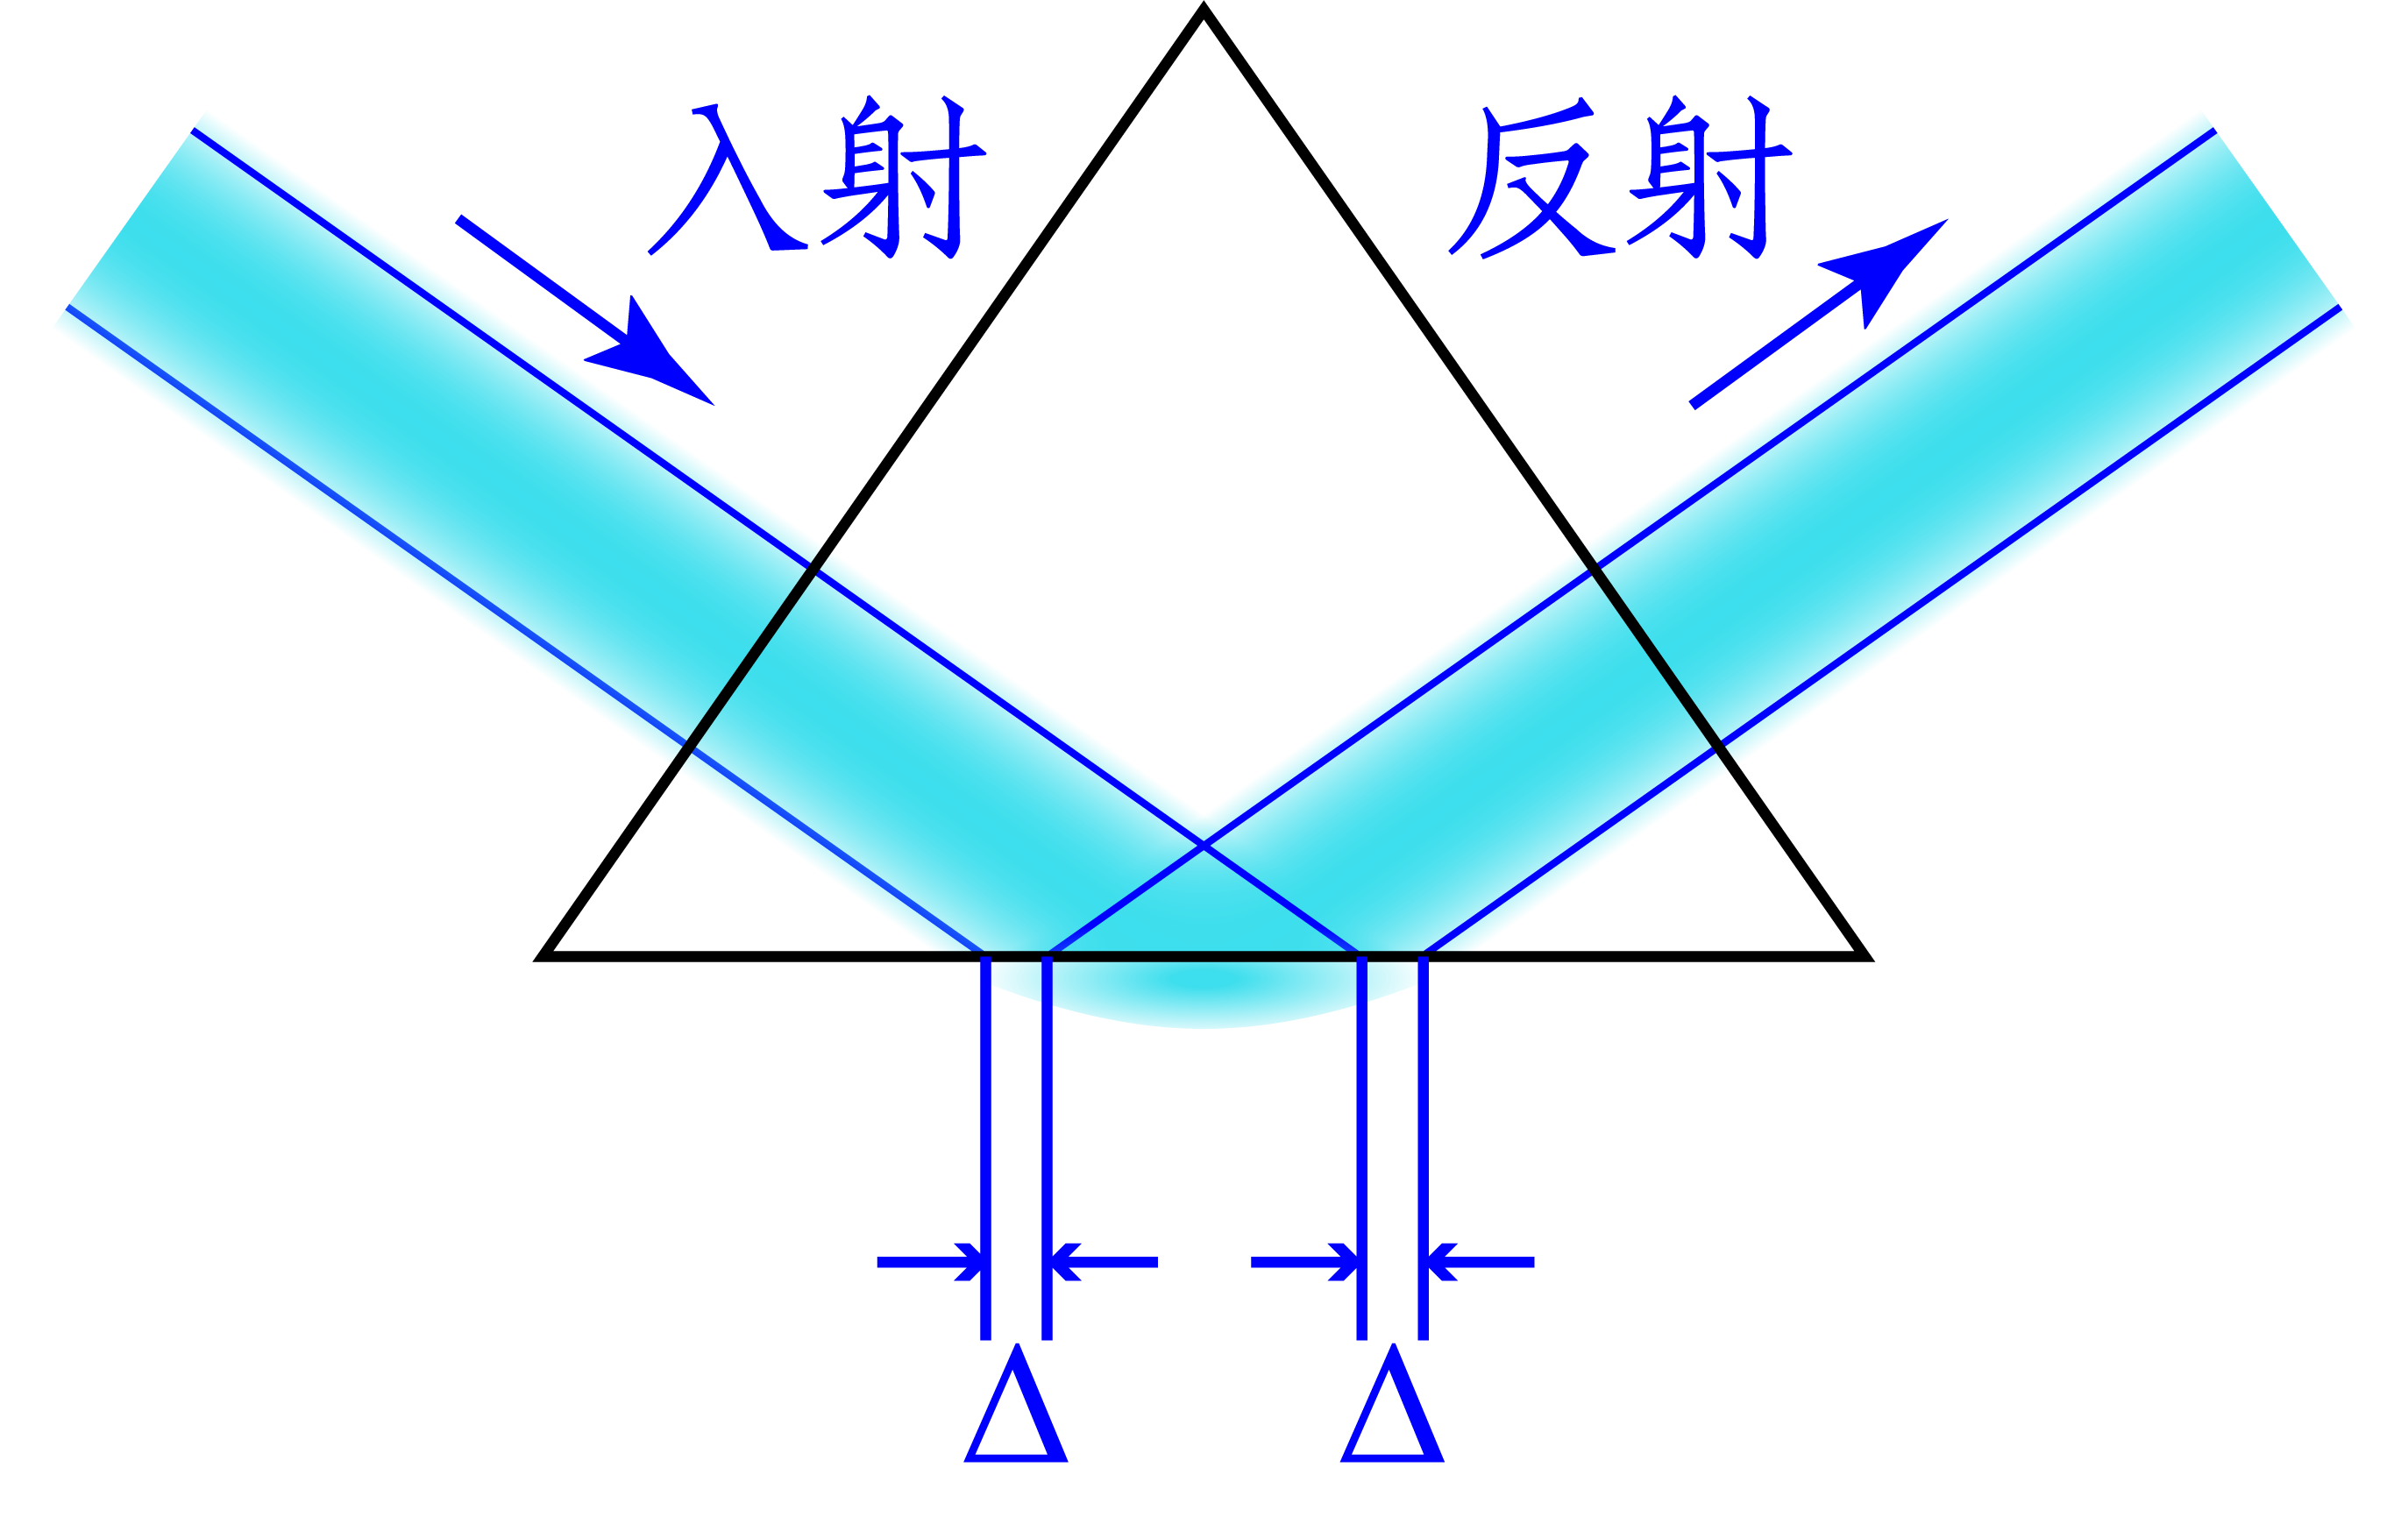
\includegraphics[width=7cm]{image/5-6-8.png}
\caption{Goos-H\"anchen Shift}
\end{wrapfigure}
值得指出,\,如果入射光并不是无限宽的平面波,\,而是可以确定其入射点位置的窄光束,\,而且也不是时刻连续的光,\,而是一个光脉冲,\,那么它的行为体现出更加有意思的结果.\,首先是著名的\emph{古斯-汉森效应}(Goos-H\"anchen effect),\,光脉冲似乎能进入下层介质,\,并在其中传播一段时间,\,随后在另一处离开下层介质出射.\,如图所示,\,这造成的前后光束中心位置的横向移位称为\emph{古斯-汉森位移}(Goos-H\"anschen shift).\,这个位移的计算需要把入射光束看成有一定角度展宽的单色平面波的叠加,\,而在入射点处恰好各个平面波相干相长,\,而光束出射点也是各个出射平面波相干相长的位置,\,不难说明:
\[\Delta_{s,p}=2\frac{\ud \delta_{s,p}}{\ud k_y}=\frac{\lambda\cos^2\delta_{s,p}}{\pi\cos\theta}\cdot\frac{\ud \tan\delta_{s,p}}{\ud \theta}\]

计算可得:
\[\Delta_s=\frac{2H\tan\theta}{n}\quad;\quad \Delta_p=\frac{\Delta_s}{(1+\frac{n^2}{n'^2})\sin^2\theta-1}\]

另一种效应是\emph{英伯特-费多罗夫效应}(Imbert-Fedorov effect).\,如果入射光是两种圆偏振光,\,那么可以证明隐失波场将具有垂直于纸面方向的能流,\,如果入射光是窄光束,\,那么反射光束将在垂直于纸面的方向发生位移,\,这个结果与光的角动量守恒相协调.\,在这里不加论述,\,详情参见光学教材.








\section{光线方程}

\subsection{光线方程与折射定律}
在给定折射率\(n\)随着空间位置连续变化的情况下,\,光将如何进行传播呢?\,把光的传播简化为光线,\,光线垂直于等相位面,\,那么\emph{光线方程}(ray equation)给出了这个问题的答案.\,这个方程写作:
\[\frac{\ud}{\ud s}(n\bs{\tau})=\nabla n\]

\begin{wrapfigure}[14]{o}[-10pt]{6cm}
\centering
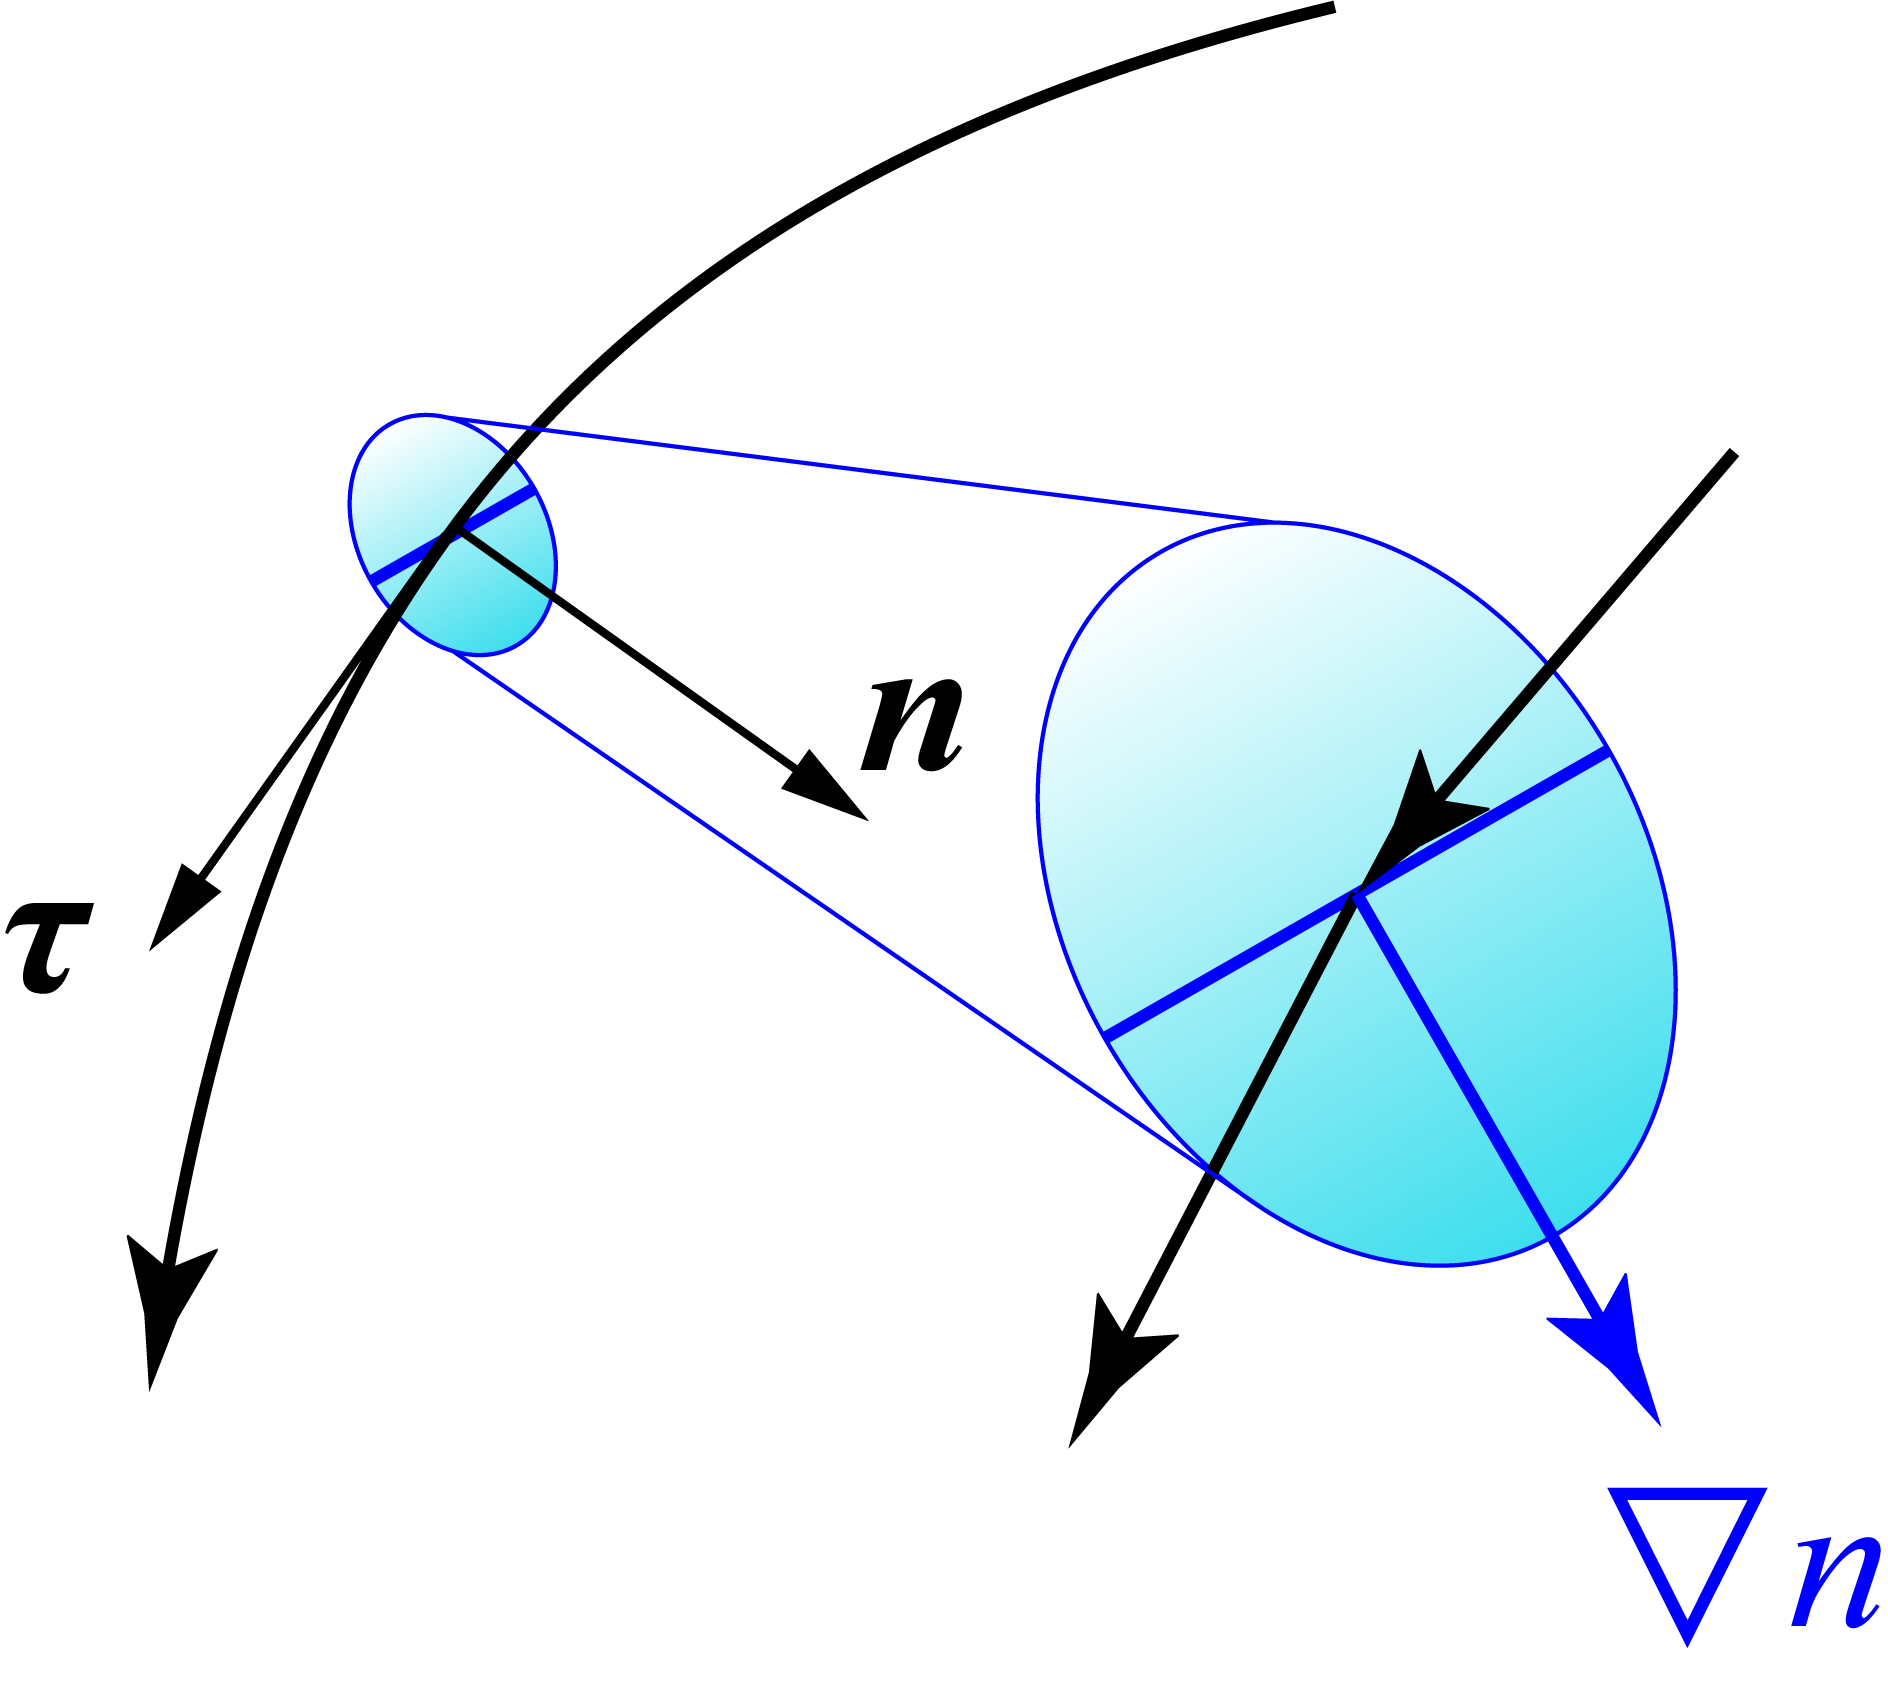
\includegraphics[width=6cm]{image/5-6-9.png}
\caption{光线方程推导}
\end{wrapfigure}
其中\(\ud s\)表示光线经过的路程.\,我们来考虑证明这个式子.\,首先我们先观察上式在法向与切向的两个分量式:
\[(\frac{\ud n}{\ud l})_\tau \bs{\tau}=(\nabla n)_\tau \bs{\tau}\]
\[n\frac{\ud \bs{\tau}}{\ud s}=n\frac{\ud \theta}{\ud s}\bs{n}=(\nabla n)_n \bs{n}\]

那么第一个式子是一个重言式(恒等式),\,而第二个式子则给出了由光线传播方向(给出了切向量\(\bs{\tau}\)与法向量\(\bs{n}\))和局域折射率分布(给出了\(\nabla n\))决定的光线弯曲程度(有曲率\(k=\dfrac{\ud \theta}{\ud s}\)描述).\,是名副其实的能够决定光线传播规律的光线方程.\,事实上,\,如图,\,如果把在该点局域处折射率分布理解为沿\(\nabla n\)的方向进行分层,\,把光线传播方向与局域统一的\(\nabla n\)方向的夹角记为\(\varphi\),\,则当光线走了\(\ud s\)时折射率变化为:
\[\ud n=\nabla n\cdot \ud s \bs{\tau}=|\nabla n|\ud s \cos\varphi\]

由折射定律:
\[\ud(n \sin\varphi)=0\quad \Rightarrow \quad \ud\varphi=-\frac{\sin\varphi\ud n}{n\cos\varphi}=-\frac{|\nabla n|}{n}\ud s\sin\varphi\]

这便是:
\[n\frac{\ud \theta}{\ud s}=n\frac{|\ud \varphi|}{\ud s}=(\nabla n)_n\]

从而给出了光线方程的表达式.

具体的,\,如果研究在二维平面上,\,折射率\(n\)仅仅与\(y\)有关而与\(x\)无关的问题,\,如稳定大气中光线的传播问题,\,此时原光线方程化为:
\[\frac{\ud}{\ud s}(n\sin\theta \bs{e}_x+n\cos\theta \bs{e}_y)=\frac{\ud n}{\ud y}\bs{e}_y\]

注意这时候我们一般取\(\theta\)为光线传播方向与界面法线(\(y\)方向)间的夹角.\,上式一方面意味着
\[n\sin\theta=\mathrm{Const.}\]

这可以看成是两层界面上折射定律的推广,\,它给出了每一个\(y\)处(因而知道\(n\))的光线传播方向,\,从而本质上余下工作只需要解出具体轨迹即可.\,只需解方程:
\[\sin\theta=\frac{1}{\sqrt{1+y'^2}}=\frac{(n_0\sin\theta_0)}{n(y)}\]

其中\((n_0\sin\theta_0)\)是根据初始条件确定的不变量.

\subsection{光力类比}
牛顿提倡光的粒子说,\,他的粒子光学理论中光粒子\footnote{与光子概念有本质区别}运动状态由位置与速度描述,\,而运动由轨迹方程与运动方程描述.\,的确,\,由光线方程可知,\,这是一个定义良好的动力学方程,\,它类似于势场中的牛顿第二定律:
\[\frac{\ud }{\ud t}(mv \bs{\tau})=-\nabla V\]

由粒子的初位置与初速度便可决定论地的给出之后的运动.\,这一种类似性为我们进行光力类比提供了良好的依据.\,然而要注意仍然有一个不同之处:\,光的速度大小不可控.\,在一个典型的光线求解的过程中,\,我们知道初始时刻的光的传播方向即可,\,而传播速度无需给出,\,事实上它也不能被改变,\,因为光速是常数,\,换一个角度理解,\,改变速度就是改变动量与能量,\,那么实际上光子的动量能量改变实际上反应在了光的颜色(频率)上.\,这是与相对论相吻合的一个结论.

那么如何进行光力类比呢?\,还是从以上两个公式的相似性出发,\,我们想象有一个质量为\(m=1\)的粒子在光的真实传播轨迹上运动,\,规定其速度为\(v=n\)\footnote{注意这不是实际光传播的相速度!\,\(v\propto n\)而\(v_g=c/n\propto 1/n\)},\,那么其受力应该为:
\[\bs{F}=\frac{\ud }{\ud t}(mv \bs{\tau})=\frac{\ud }{\ud s/v}(n \bs{\tau})=v\nabla n=n\nabla n=-\nabla(-\frac{n^2}{2})\]

也就是说如果认为粒子是在\(V=-\dfrac{n^2}{2}\)的势场中运动的,\,那么其模仿光线的轨迹与用该处折射率来定标自己的运动速度的做法又恰巧是符合动力学规律的.\,恰巧,\,这个运动的守恒能量:
\[E=T+V=\frac{v^2}{2}-\frac{n^2}{2}=0\]

光粒子的运动只能是能量为零的,\,如果忽略光的色散,\,那么不同频率的光在同一个折射率场中将具有完全相同的传播轨迹,\,实际上没有光粒子运动的``快慢''的说法.

我们总结光力类比法求光线传播问题的大意:

\begin{enumerate}
	\item 明确折射率场分布\(n(\bs{r})\),\,明确光线初始入射位置与方向\(\bs{\tau}_0(\bs{r}_0)\).
	\item 光力类比:\,设置势场\(V(\bs{r})=-\dfrac{n^2}{2}\),\,设置粒子,\,质量为\(1\),\,初始位置\(\bs{r}_0\),\,速度\(\bs{v}_0=n\bs{\tau}_0\).
	\item 求解粒子的运动,\,得出运动轨迹.
	\item 这个轨迹也就是光线的轨迹,\,再由已知的轨迹求解其他问题(如传播时间等).
\end{enumerate}

这种方法往往是方便的,\,它会使得很多我们在力学问题中有明确结论的结果可以直观地呈示出来.\,例如在之前的折射率随\(y\)改变的情形,\,它对应着水平方向平移对称的势场,\,从而有\(x\)方向的动量守恒,\,这就是:
\[n\sin\theta=\mathrm{Const.}\]

同样的道理,\,如果光线在一个球对称的折射率场\(n(r)\)中运动时,\,其轨迹恰好对应有心力场中粒子运动的轨迹.\,例如取:
\[V=-\frac{k}{r}+C\quad\Rightarrow\quad n=n_0\sqrt{\frac{2a}{r}-1}\]

那么这个粒子的运动是在环域\(0<r<2a\)上的椭圆,\,而且计算可以表明改变初始条件,\,其半长轴固定为\(a\),\,保证其轨迹范围不会超过这个环域.

而此时应该有角动量守恒,\,用光线方向与径向夹角\(\theta\)表示则为:
\[nr\sin\theta=L=\mathrm{Const.}\]

\section{费马原理}
\begin{wrapfigure}[14]{o}[-10pt]{6cm}
\centering
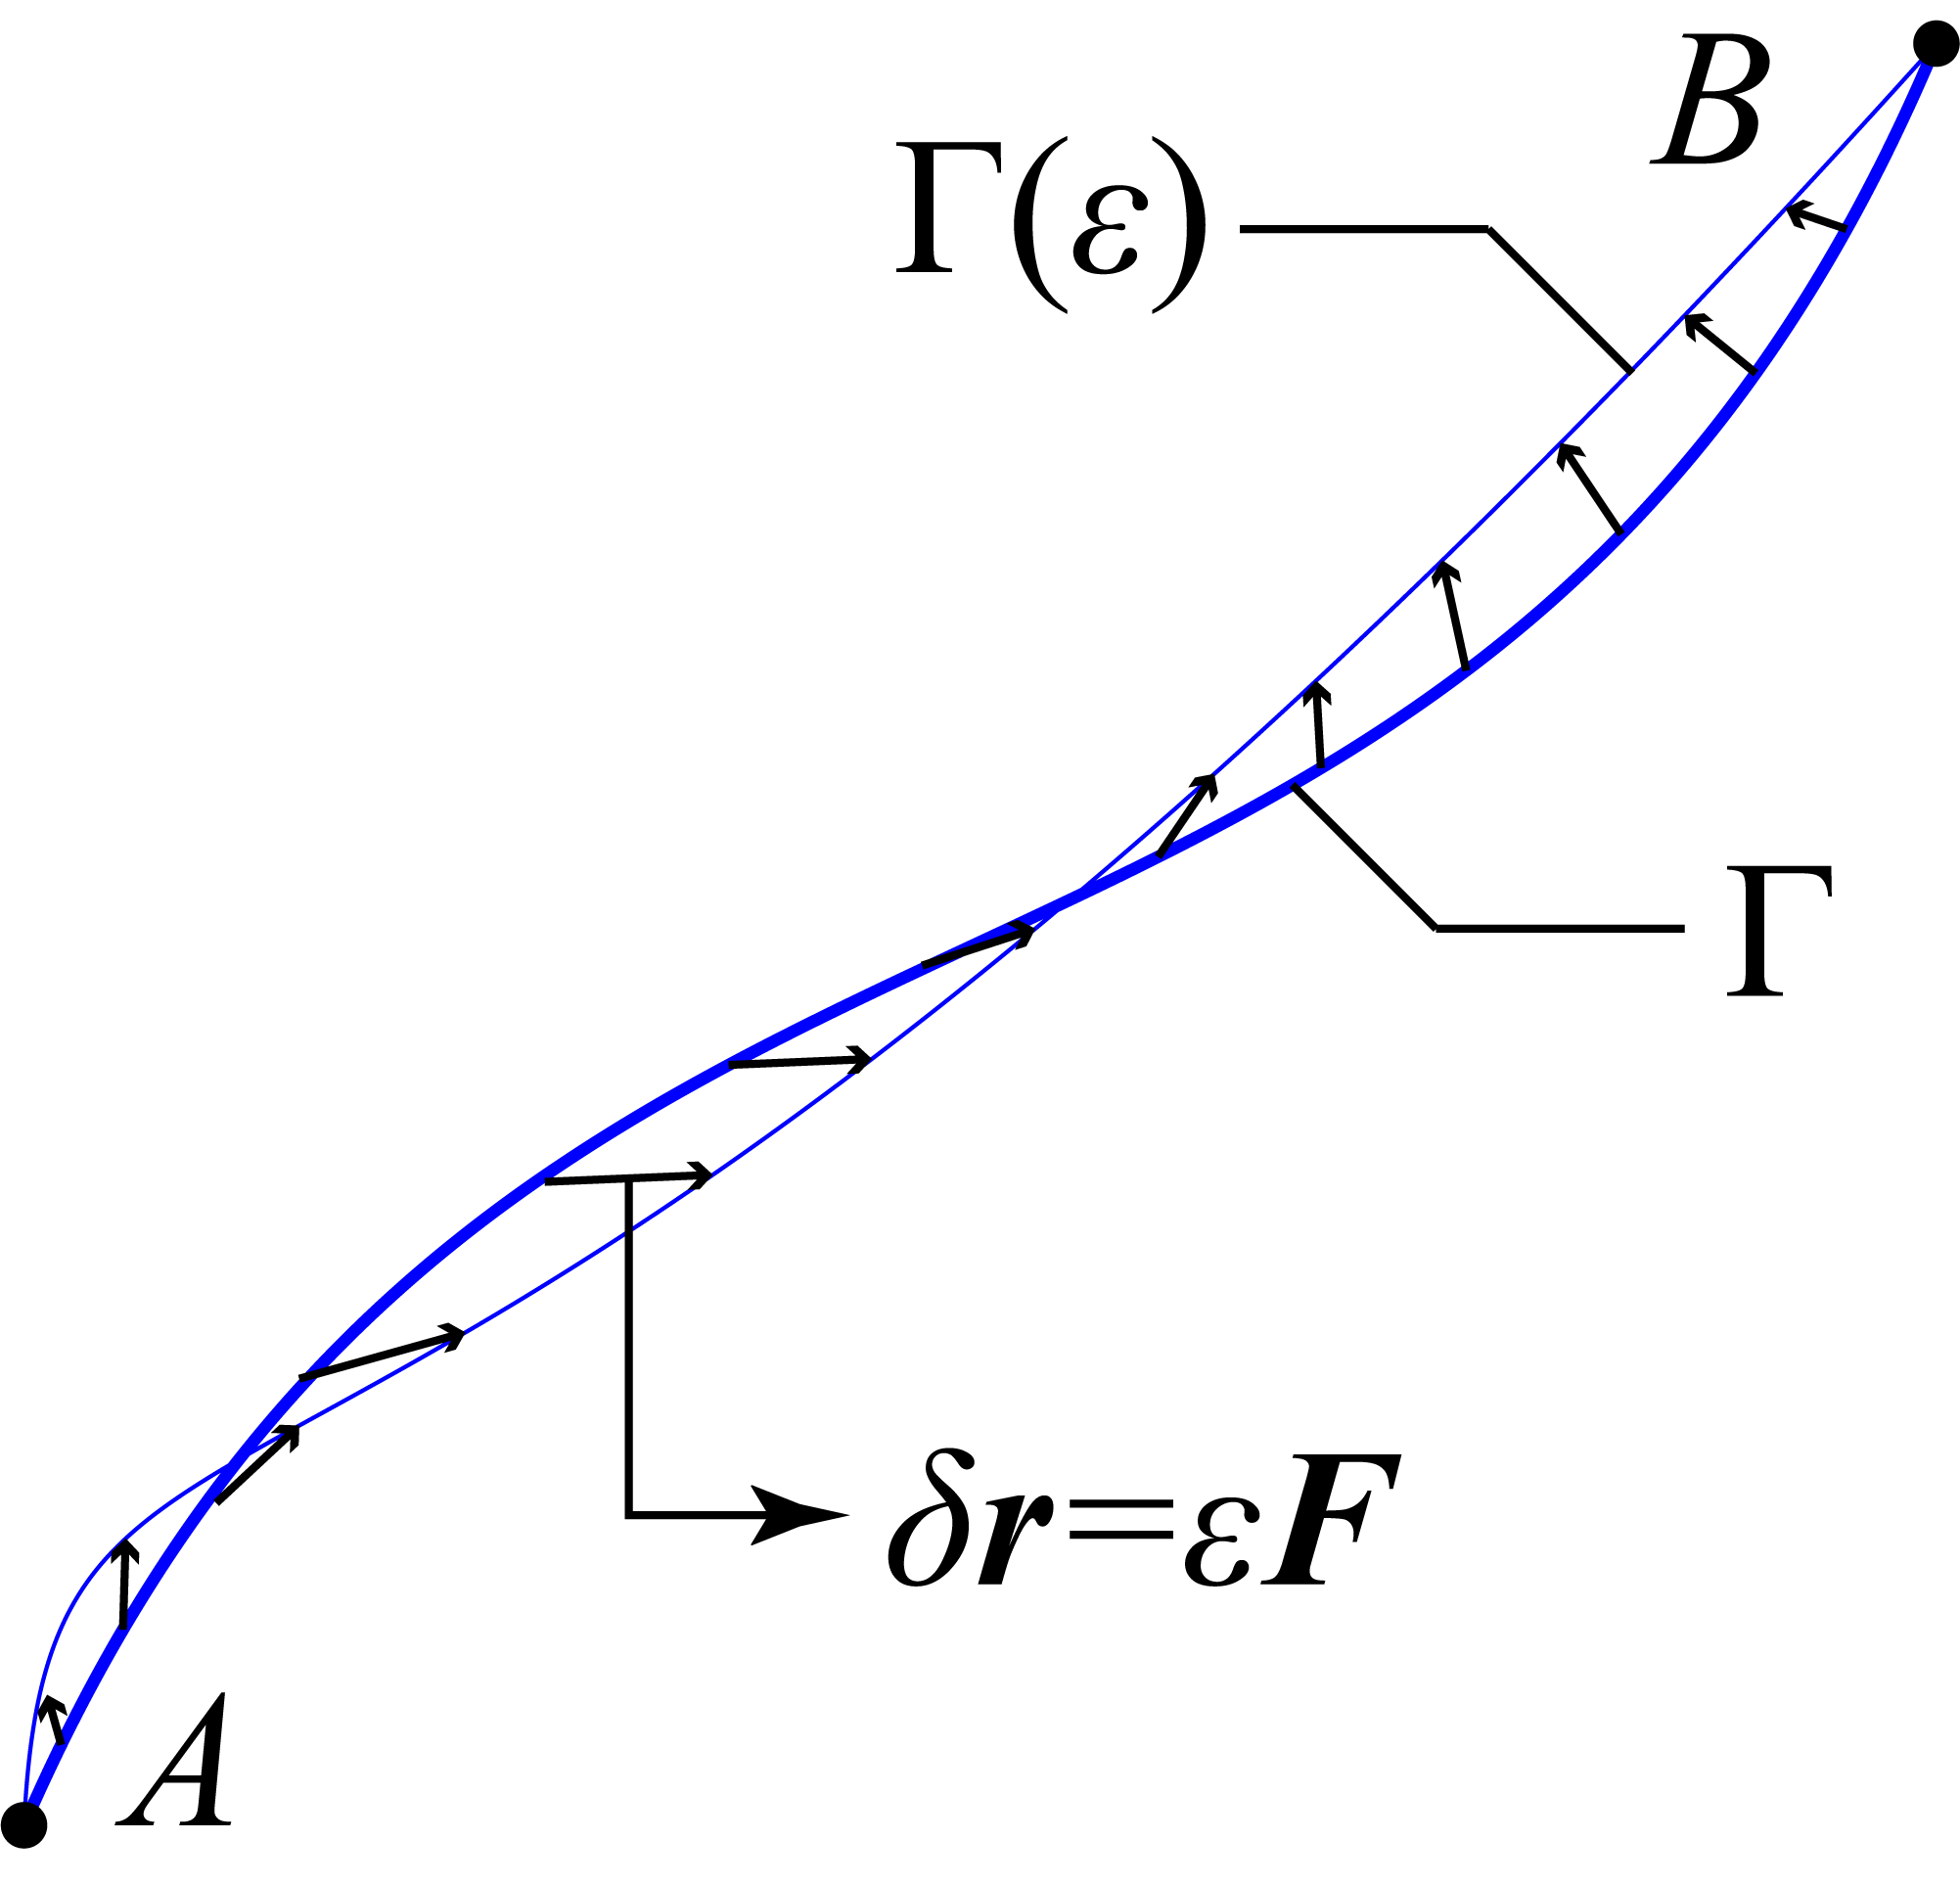
\includegraphics[width=6cm]{image/5-6-10.png}
\caption{光程变分}
\end{wrapfigure}
类似于力学变分原理,\,光线方程的存在也意味着光学的变分原理,\,这个原理即为著名的费马原理:
\[\delta\int_A^B n\ud s=0,\;{\rm if}\;\delta\bs{r}_A=0{\rm \; and \;}\delta\bs{r}_B=0\]

如何理解这个原理呢,\,首先这个折射率对路程的积分称为\emph{光程}(optical path),\,在光力类比下它实际上就是满足能量守恒条件下的相积分:
\[S=\int_{A\xrightarrow{\Gamma} B} n\ud s=\int_{A\xrightarrow{\Gamma} B} \bs{p}\cdot\ud \bs{r}\]

而从\(A\)点到\(B\)点的光传播可以由某种参数方程描述:
\[\Gamma :\quad\bs{r}=\bs{R}(t),\,\bs{R}(t_A)=\bs{r}_A,\,\bs{R}(t_B)=\bs{r}_B\]

而变分的意思是我们另取一种可能的轨迹,\,比如:
\[\Gamma(\epsilon):\quad(\bs{r}+\delta\bs{r})(t)=\bs{R}(t)+\epsilon \bs{F}(t)\]

那么费马原理要求在轨迹端点不变的条件下,\,新的光程关于所有可能的微扰方向\(\bs{F}(t)\),\,关于其微扰强度的一阶导数都要等于零:
\[S(\epsilon)=\int_{A\xrightarrow{\Gamma(\epsilon)} B} n\ud s\quad ;\quad \left.\frac{\ud S(\epsilon)}{\ud \epsilon}\right|_{\epsilon=0}=0\]

这个原理是等价于光线方程的,\,证明这一点需要用到较为专门的矢量分析技巧,\,在此略去.\,用文字一般可以表述为:

\begin{quote}
两点之间光线的实际轨迹,\,是光程取平稳值的路径.
\end{quote}

\begin{wrapfigure}[14]{o}[-10pt]{6cm}
\centering
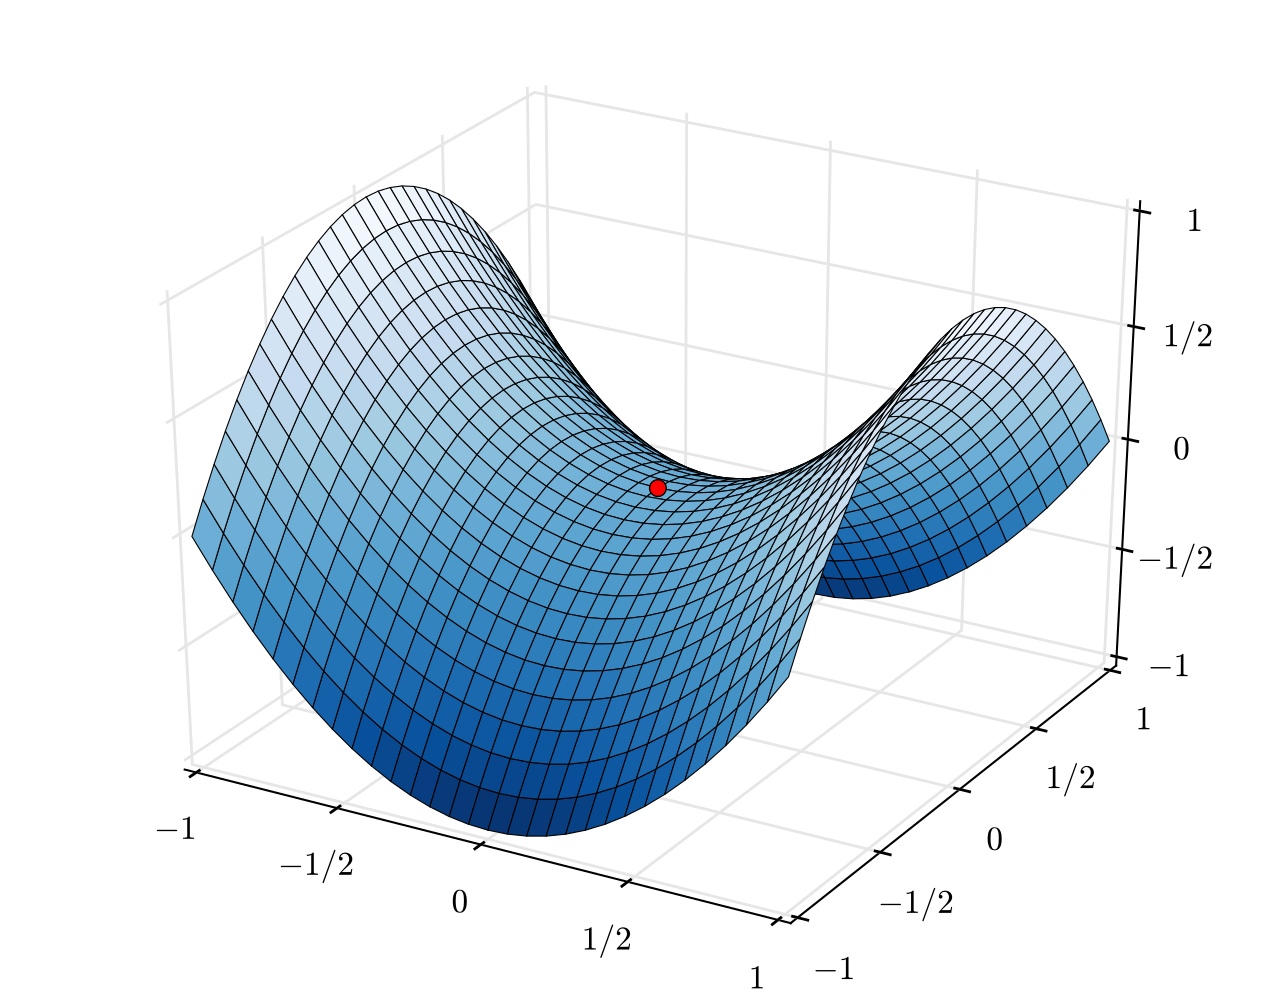
\includegraphics[width=6cm]{image/5-6-11.png}
\caption{二维鞍点处势取平稳值}
\end{wrapfigure}
其中的``平稳值''的说法,\,既包含了极大,\,也包含了极小,\,还包含了一些复合的情况,\,比如如图,\,我们考虑一个马鞍面上有一个质点在鞍点处于平衡状态,\,那么在一个方向上势能最高,\,另一个方向上势能最低,\,然而该点能平衡,\,因为势能取得了``平稳值''.\,二自由度下已经出现了两个自由度方向微扰后极大极小性质出现差异的情形,\,而光程问题则是在所有可能的轨迹空间中进行无穷多自由度的微扰的问题,\,普遍来说符合之前我们定义的一阶变分为零即可以符合费马原理的条件,\,故冠以``平稳值''的说法.

最后,\,值得指出以上结论都是在波动理论尚未发展到一定程度时的替代性的粒子理论.\,在有了波动理论以后以上两个结论都将得到极为简单的解释.\,我们把变折射率问题中的光的等相位面找到,\,光线即将垂直于等相位面.\,而相位场\footnote{在粒子论里称为\emph{程函}(eikonal)}\(\varphi(\bs{r})\)与光传播方向,\,折射率间关系即为:
\[\nabla\varphi=\bs{k}=k_0 n\bs{\tau}\]

该式两边同时对传播方向取方向导数:
\[\frac{\ud}{\ud s}(\nabla\varphi)=k_0\frac{\ud}{\ud s}(n\bs{\tau})\]

而此式左边,\,在沿传播方向求的导数应该理解为与下一个梯度算符独立的,\,故可以交换顺序:
\[\frac{\ud}{\ud s}(\nabla\varphi)=\nabla(\frac{\ud \varphi}{\ud s})=\nabla{k}=k_0\nabla{n}\]

两式联立便得到光线方程:
\[\frac{\ud}{\ud s}(n\bs{\tau})=\nabla n\]

而费马定理也非常容易理解:\,光程积分:
\[\int n\ud s=\int n\bs{\tau}\cdot \ud \bs{r}=\frac{1}{k_0}\int \nabla \varphi\cdot \ud \bs{r}=\frac{\Delta \varphi}{k_0}\]

所以在光程微扰下只要起点与终点固定,\,光程就不会有改变.
